\documentclass[11pt]{report}

\usepackage{a4wide}
\usepackage[T2A]{fontenc}
\usepackage[utf8]{inputenc}
\usepackage[main=russian, english]{babel}
\usepackage{graphicx}
\usepackage{amsmath}
\usepackage{amsthm}
\usepackage{amssymb}
\usepackage{amsfonts}
\usepackage{mathtools}
\usepackage{cases}
\usepackage{hyperref}
\usepackage{indentfirst}
\usepackage{float}
\usepackage{subcaption}
\usepackage{tocloft}
%\usepackage[nottoc,numbib]{tocbibind}
\usepackage{epstopdf} % to change .eps to .pdf
\epstopdfsetup{update} % conversion only if no .pdf file already created

\graphicspath{{./images}}

%\setlength{\cftsecindent}{0pt}% Remove indent for \section
%\setlength{\cftsubsecindent}{0pt}% Remove indent for \subsection

\DeclareMathOperator{\Bin}{Bin}
\DeclareMathOperator{\Be}{Be}
\DeclareMathOperator{\Geom}{Geom}
\DeclareMathOperator{\Exp}{Exp}
\DeclareMathOperator{\Pois}{Pois}

\begin{document}

\thispagestyle{empty}

\begin{center}
\ \vspace{-3cm}


\includegraphics[width=0.5\textwidth]{msu.eps}\\
{\scshape Московский государственный университет имени М.~В.~Ломоносова}\\
Факультет вычислительной математики и кибернетики\\
Кафедра системного анализа

\vfill

{\LARGE Отчёт по практикуму}

\vspace{1cm}

{\Huge\bfseries <<Стохастический анализ и моделирование>>}
\end{center}

\vspace{1cm}

\begin{flushright}
  \large
  \textit{Студент 415 группы}\\
  А.\,А.~Пилюшенок

  \vspace{5mm}

  \textit{Руководитель практикума}\\
  д.ф.-м.н., профессор С.\,Н.~Смирнов
\end{flushright}

\vfill

\begin{center}
Москва, 2024
\end{center}

% Custom Commands start here
%\let\oldref\ref
%\renewcommand{\ref}[1]{(\oldref{#1})}
\renewcommand{\phi}{\varphi}
\renewcommand{\sh}{\operatorname{sh}}
\renewcommand{\phi}{\varphi}
\renewcommand{\tilde}{\widetilde}
\newcommand{\eps}{\varepsilon}
\newcommand{\const}{\operatorname{const}}
\newcommand{\atan}[1]{\operatorname{arctg}{#1}}
\newcommand{\mo}{\mathbb{E}}
\newcommand{\di}{\mathbb{D}}
\newcommand{\p}{\mathbb{P}}

\newtheorem{theorem}{Теорема}
\newtheorem{definition}{Определение}
\newtheorem{statement}{Утверждение}

\newpage % ToC starts here

\tableofcontents

\newpage % Main document starts here

\chapter{Первая часть практикума}

\section{Задание 1}

\subsection{Условие}

\begin{enumerate}
\item Реализовать генератор схемы Бернулли с заданной вероятностью успеха $p$. На основе генератора схемы Бернулли построить датчик биномиального распределения.
\item Реализовать генератор геометрического распределения; проверить для данного распределения свойство отсутствия памяти.
\item Промоделировать игру в орлянку: бесконечную последовательность независимых испытаний Бернулли 
с бросанием “правильной” (честной, $p=0.5$) монеты. Величина “выигрыша” $S_n$ определяется как сумма 
по $n$ испытаниям значений 1 и -1 в зависимости от выпавшей стороны монеты. Проиллюстрировать в виде
ломаной поведение нормированной суммы $Y(i)=\frac{S_i}{\sqrt{n}}$ как функцию от номера испытания $i$ 
для отдельно взятой траектории. Дать теоретическую оценку для значения $Y(n)$ при $n\to\infty$.
\end{enumerate}

\subsection{Генераторы схемы Бернулли и биномиального распределения}

Дадим описание схемы Бернулли на метаязыке.

\begin{definition}
Схемой Бернулли с вероятностью $p$ называется эксперимент, состоящий из последовательности испытаний, обладающих следующими свойствами:
\begin{itemize}
    \item воспроизводимость --- все испытания проходят в подобных (может, не полностью идентичных) условиях;
    \item отсутствие взаимного влияния;
    \item каждому испытанию сопоставляется численная характеристика, которая реализуется (''успех`` с вероятностью $p$) или не реализуется (``неуспех'' с вероятностью $1-p$).
\end{itemize}
\end{definition}

\begin{definition}
Рассмотрим схему Бернулли с вероятностью $p$, состоящую из $n$ последовательных испытаний. Тогда распределение числа ``успехов'' в такой схеме Бернулли называется биномиальным с числом испытаний $n$ и вероятностью $p$.
\end{definition}

Для моделирования случайных величин, имеющих распределение Бернулли с параметром $p$ (отвечает схеме Бернулли с единственным испытанием), воспользуемся методом обращения функции распределения. Он основан на следующем утверждении.

\begin{statement}
Пусть функция распределения $F(\cdot)$ имеет обратную $F^{-1}(\cdot)$. Положим $\nu\sim\mathrm{U}[0,1]$. Тогда функцией распределения случайной величины $\xi=F^{-1}(\nu)$ является $F(\cdot)$.
\end{statement}
\begin{proof}
$$
F_\xi(x) = \mathbb{P}(\xi < x) = \mathbb{P}(F^{-1}(\nu) < x) = \mathbb{P}(\nu < F(x)) = F(x).
$$
\end{proof}



\begin{statement}
Биномиальное распределение $\mathrm{Bin}(n,p)$ можно представить как сумму $n$ н.о.р.с.в., имеющих распределение $\mathrm{Be}(p)$.
\end{statement}
\begin{proof}
Пусть $\xi_i\sim\Be(p),~i=\overline{1,n}$ и $\eta\sim\Bin(n,p)$. Тогда
\[
\p(\eta = k) = C_n^kp^k(1-p)^{n-k},\quad k=\overline{0,n}.
\]
Покажем методом математической индукции, что 
\[
\p(\eta = k) = \p\left(\sum_{l=1}^n\xi_l = k\right),\quad k=\overline{0,n}.
\]
\begin{itemize}
\item При $n=1$:
\[
\p(\eta = 0) = 1-p, \quad\p(\eta = 1) = p.
\]
т.е., $\eta\sim\Be(p)\equiv\Bin(1,p)$.
\item Пусть верно для $n$, покажем, что верно для $n+1$:
\begin{gather*}
% \p(\eta = k) &= C_n^kp^k(1-p)^k. \\
\p\left(\sum^{n+1}_{l=1}\xi_l=k\right) = 
\p\left(\sum^{n}_{l=1}\xi_l=k~\bigg|~\xi_{n+1}=0\right)\cdot
\p(\xi_{n+1}=0) + \\
+ \p\left(\sum^{n}_{l=1}\xi_l=k-1~\bigg|~\xi_{n+1}=1\right)\cdot
\p(\xi_{n+1}=1) = \\
= (C_n^kp^k(1-p)^{n-k})\cdot (1-p) + (C_n^{k-1}p^{k-1}(1-p)^{n-(k-1)})\cdot p = \\
= (C_n^k + C_n^{k-1})\cdot p^{k}(1-p)^{n+1-k}.
\end{gather*}
Далее воспользуемся тождеством Вандермонда $C_n^k + C_n^{k-1} = C_{n+1}^k$ и получим требуемое.
\end{itemize}
\end{proof}

На графиках \ref{fig:bern}, \ref{fig:bin-clt} продемонстрирована работа датчиков. Для биномиального распределения показана справедливость Центральной Предельной Теоремы (формулировка приведена в пункте \ref{ss:coin-toss}), где $\mu = np, \sigma^2 = np(1-p)$ --- характеристики биномиального распределения.

\begin{figure}[H]
    \centering
    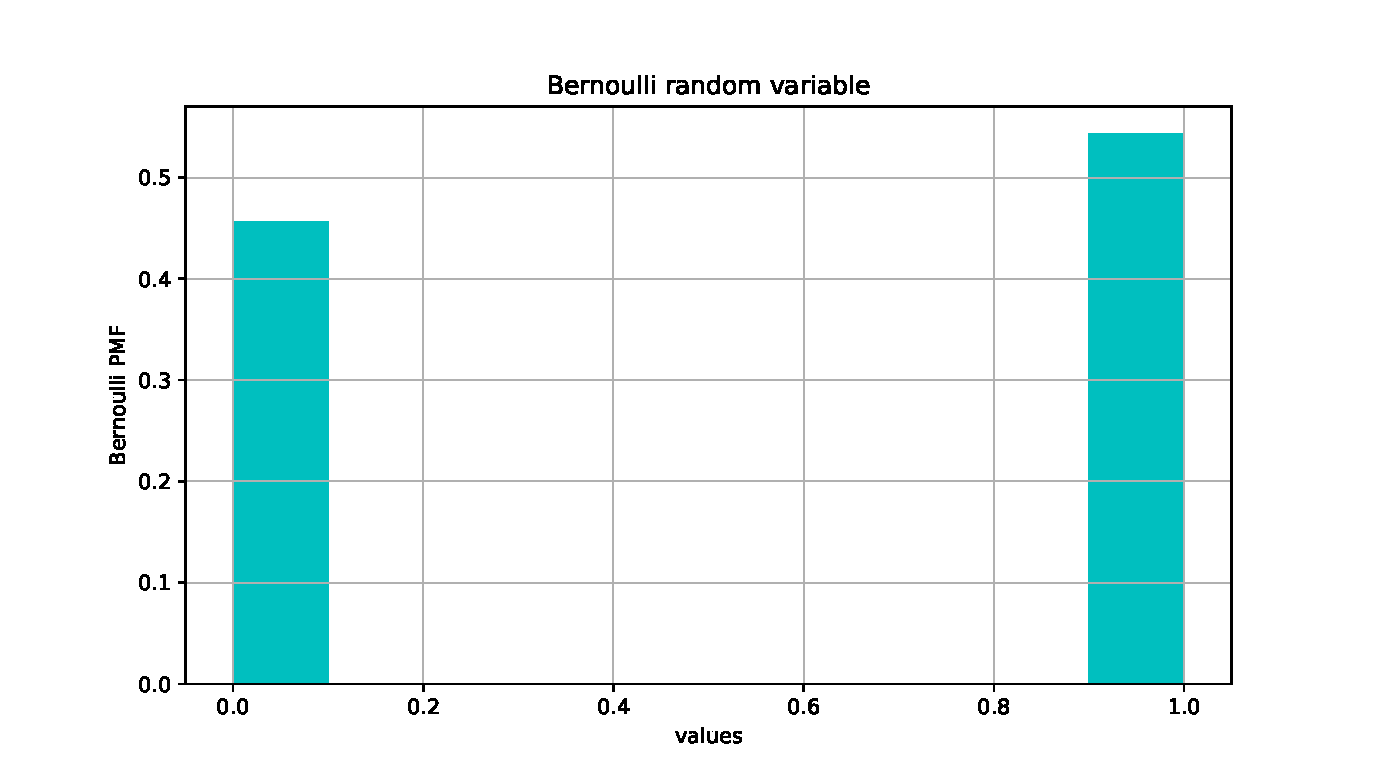
\includegraphics[width=0.9\linewidth]{bern.eps}
    \caption{Выборка распределения Бернулли $p=0.54321$ размера $N=10^7$.}
    \label{fig:bern}
\end{figure}

\begin{figure}[H]
    \centering
    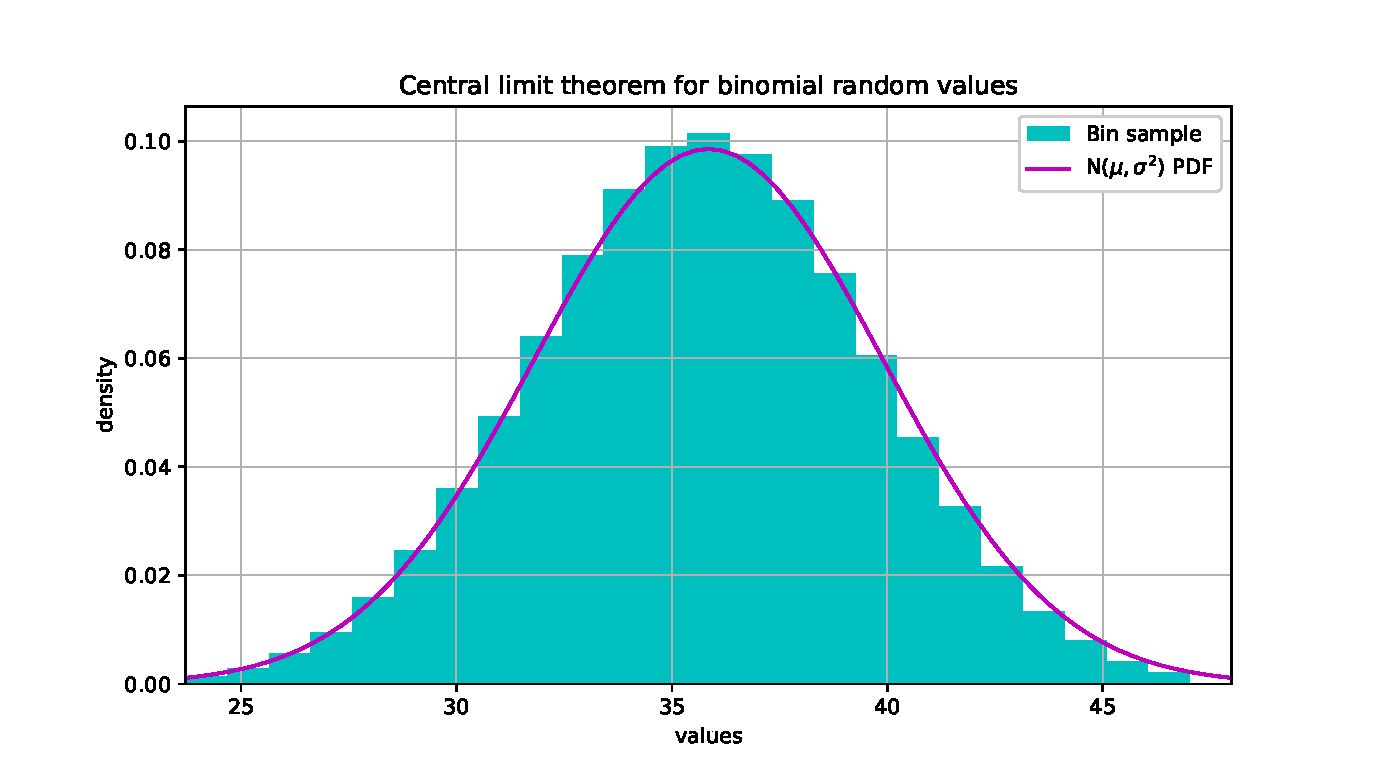
\includegraphics[width=0.9\linewidth]{bin-clt.eps}
    \caption{Выборка биномиального распределения $n=66, p=0.54321$ размера $N=10^6$.}
    \label{fig:bin-clt}
\end{figure}

\subsection{Генератор геометрического распределения}\label{ss:geom}

\begin{definition}
Геометрическое распределение - это распределение числа неуспехов до первого успеха в схеме Бернулли с неограниченным числом испытаний.
\end{definition}

Обозначим
\begin{gather*}
\xi \sim \operatorname{Geom}(p),\quad \nu \sim \operatorname{U}[0,1].\\
\mathbb{P}(\xi = n) = p(1-p)^n,\quad \sum_{k=0}^{n} p(1-p)^k = 1 - (1-p)^{n+1} = s_{n+1}.
\end{gather*}
Пользуясь генератором равномерного распределения, реализуем генератор геометрического распределения, исходя из следующих соображений:
$$
\mathbb{P}(\xi = n) = \mathbb{P}(s_{n}<\nu\leqslant s_{n+1}) = \mathbb{P}((1-p)^{n+1} \leqslant 1-\nu < (1-p)^{n}).
$$
$$
\Longrightarrow~ \boxed{\mathbb{P}(\xi = n) = \mathbb{P}\left( n < \dfrac{\ln{(1-\nu)}}{\ln(1-p)} \leqslant n+1  \right).}
$$
Отметим, что $(1-\nu) \sim \operatorname{U}[0,1]$.

Таким образом, будем моделировать случайную величину
$$
\eta = \bigg\lfloor \dfrac{\ln\nu}{\ln(1-p)} \bigg\rfloor.
$$

Можно доказать, что $\frac{\ln\nu}{\ln(1-p)}\sim\mathrm{Exp}(\ln\frac{1}{1-p})$:
$$
\mathbb{P}\left(\frac{\ln\nu}{\ln(1-p)}<x\right) = \mathbb{P}(\nu < e^{\ln(1-p)x}) = 1 - e^{\ln(1-p)x}.
$$

\begin{statement}
Геометрическое распределение с параметром $p$ обладает свойством отсутствия памяти:
$$
\mathbb{P}(\xi > m+n ~\vert~ \xi \geqslant m) = \mathbb{P}(\xi > n),\quad \forall m,n \in \{0,1,2\dots\}
$$
\end{statement}
\begin{proof}
\begin{gather*}
\mathbb{P}(\xi > m+n ~\vert~ \xi \geqslant m) = \dfrac{\mathbb{P}(\xi > m+n)}{\p(\xi \geqslant m)} = \dfrac{\sum\limits^{\infty}_{k=m+n+1}p(1-p)^k}{\sum\limits^{\infty}_{k=m}p(1-p)^k} = \\
= \dfrac{p\frac{(1-p)^{m+n+1}}{p}}{p\frac{(1-p)^{m}}{p}} = (1-p)^{n+1} = \p(\xi>n).
\end{gather*}
\end{proof}



Чтобы проверить этот результат численно, построим две гистограммы для двух выборок (отвечающих левой и правой частям соответственно).
Сдвинутые графики должны совпасть. На рисунке \ref{fig:geom-memo} продемонстрирован теоретический результат.

\begin{figure}[H]
    \centering
    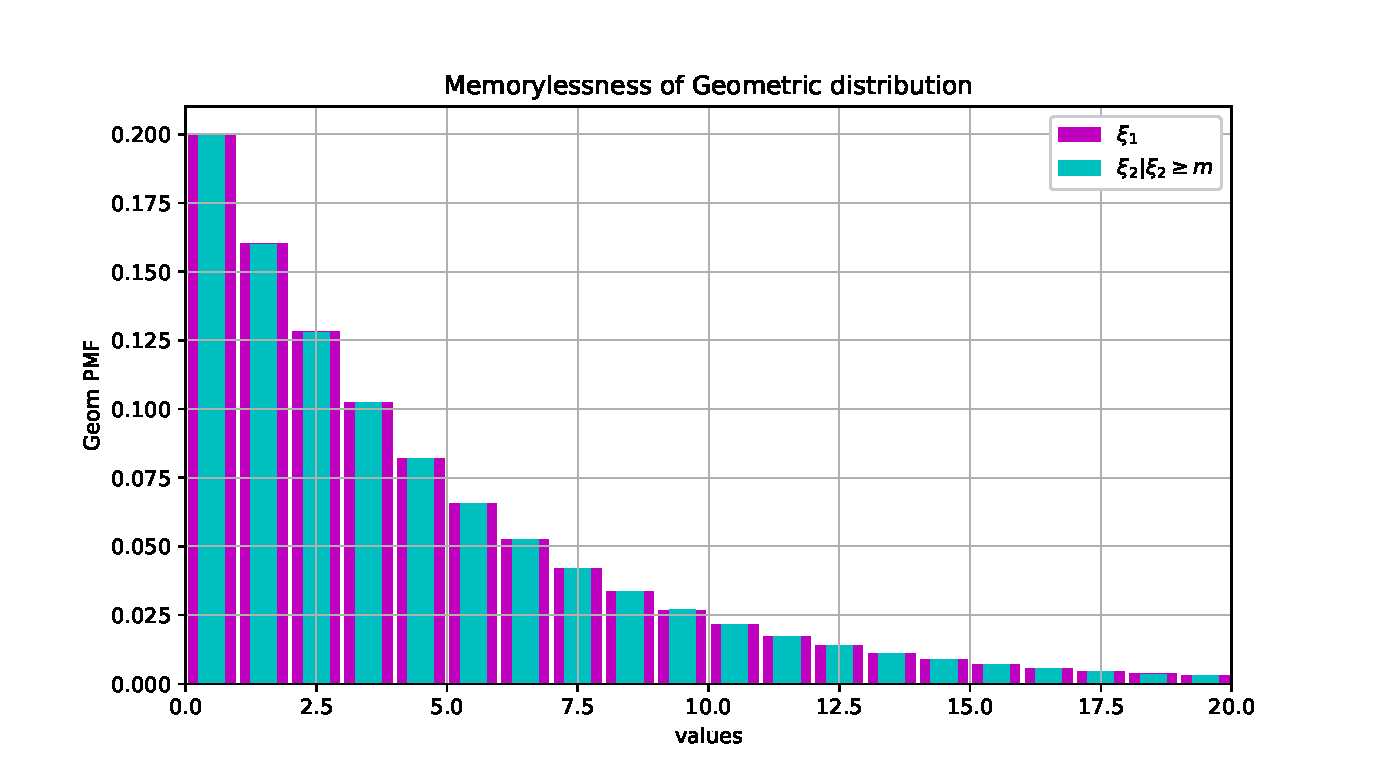
\includegraphics[width=0.9\linewidth]{geom-memo.eps}
    \caption{Проверка отсутствия памяти $\Geom(p), p=0.2, m=7$ на выборках размера $N=10^7$.}
    \label{fig:geom-memo}
\end{figure}

\subsection{Игра в орлянку}\label{ss:coin-toss}

 \begin{theorem}[центральная предельная теорема для независимых одинаково распределенных случайных величин]
Пусть $X_1,X_2,\dots$ - последовательность н.о.р. (невырожденных) случайных величин с конечным вторым моментом.
Пусть $S_n = \sum_{k=1}^{n}X_k$. Тогда
$$
\lim_{n\to\infty}\mathbb{P}\left( \dfrac{S_n-\mathbb{E}S_n}{\sqrt{\mathbb{D}S_n}} < x \right) = \mathrm{\Phi}(x) = \dfrac{1}{\sqrt{2\pi}} \int_{-\infty}^x e^{-\frac{x^2}{2}}dx.
$$
\end{theorem}
\begin{proof} Приведено в \cite{shiryaev-1} с.447-449 \end{proof}

Рассмотрим
$$
S_n = \sum^{n}_{i=1} \eta_i,\quad \eta_i = 2\xi_i-1,\quad \xi_i \sim \operatorname{Be}(p) \text{ --- i.i.d.r.v.}\\
Y_n = \dfrac{S_n}{\sqrt{n}}.
$$

Зафиксируем $p=1/2$. В таком случае
$$
\mathbb{E}\nu_i \equiv \mu = 2p-1 = 0.\\
\mathbb{D}\nu_i \equiv \sigma^2 = 4p(1-p) = 1.
$$

Воспользуемся ЦПТ.
$$
\mathbb{P}\left( \dfrac{S_n - n\mu}{\sigma\sqrt{n}} < x \right) \to \Phi(x)=\dfrac{1}{\sqrt{2\pi}}\int_{-\infty}^{x}e^{-y^2/2}dy,~n\to\infty.
$$

Заметим, что нормированная случайная величина внутри функции распределения в левой части выражения совпадает с $Y_n$. \
Также отметим, что третий абсолютный момент $\mathbb{E}|\eta_i|^3=1$, ведь $|\eta_i|\equiv1$. \
В таком случае можем воспользоваться неравенством Берри-Эссеена, где $c_0\in(0.4,0.5)$.
$$
\sup_{x\in\mathbb{R}}\left| \mathbb{P}\left( \dfrac{S_n}{\sqrt{n}} < x \right) - \Phi(x) \right| < \dfrac{c_0}{n^{3/2}}.
$$

Получили оценку скорости сходимости в ЦПТ.
Нас также интересует оценка значений $Y_n(\omega)$.

Уже показали, что
$$
Y_n \stackrel{d}{\to} \xi\sim\mathrm{N}(0,1).
$$
Следовательно, по мере увеличения числа элементов $n$ нормированная сумма $Y(n)$ будет распределена нормально.

Также продемонстрируем поведение траектории $Y_i = \frac{S_i}{\sqrt{n}},~ i=\overline{0,n}$.

\begin{figure}[H]
    \centering
    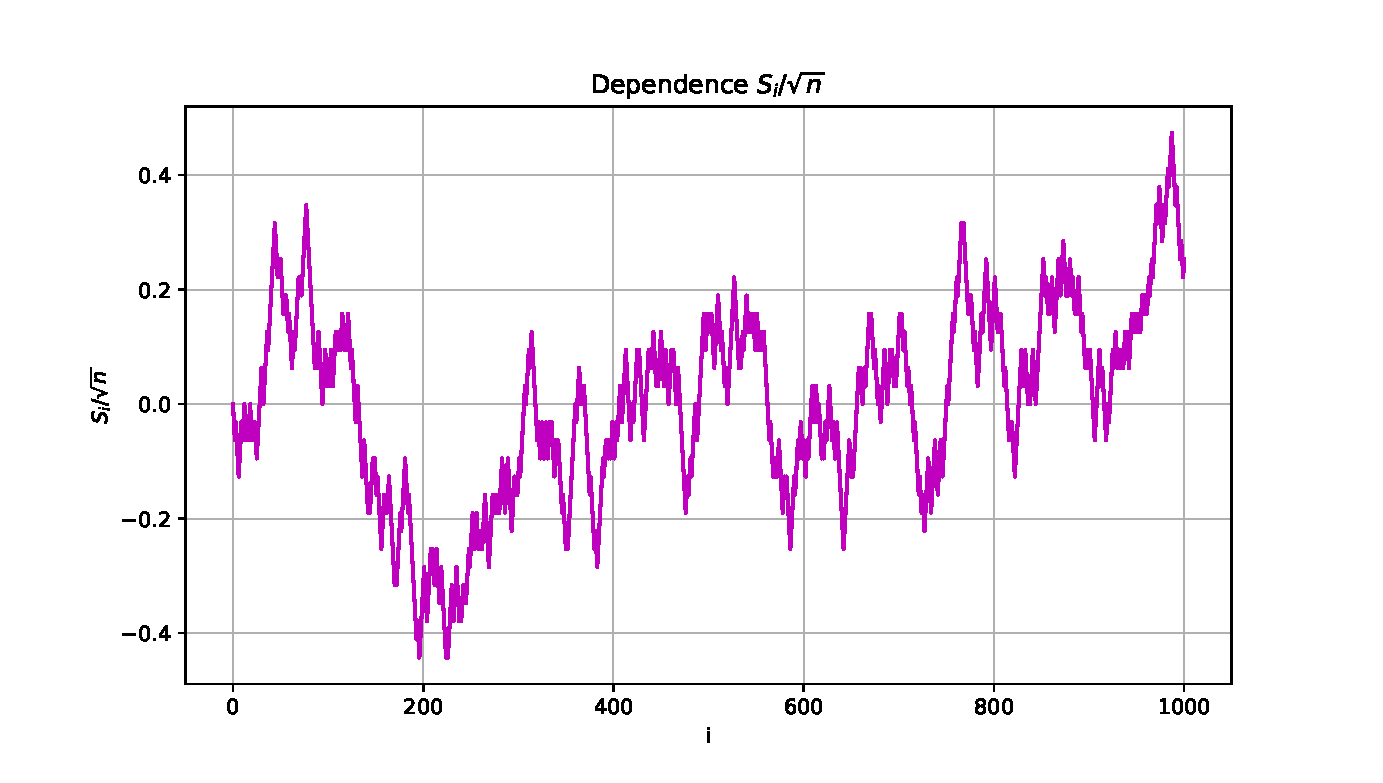
\includegraphics[width=0.9\linewidth]{coin-toss-dep.eps}
    \caption{Зависимость $Y_i=S_i/\sqrt{n},i=\overline{0,n}, n=1000$.}
    \label{fig:coin-toss-dep}
\end{figure}

\begin{figure}[H]
    \centering
    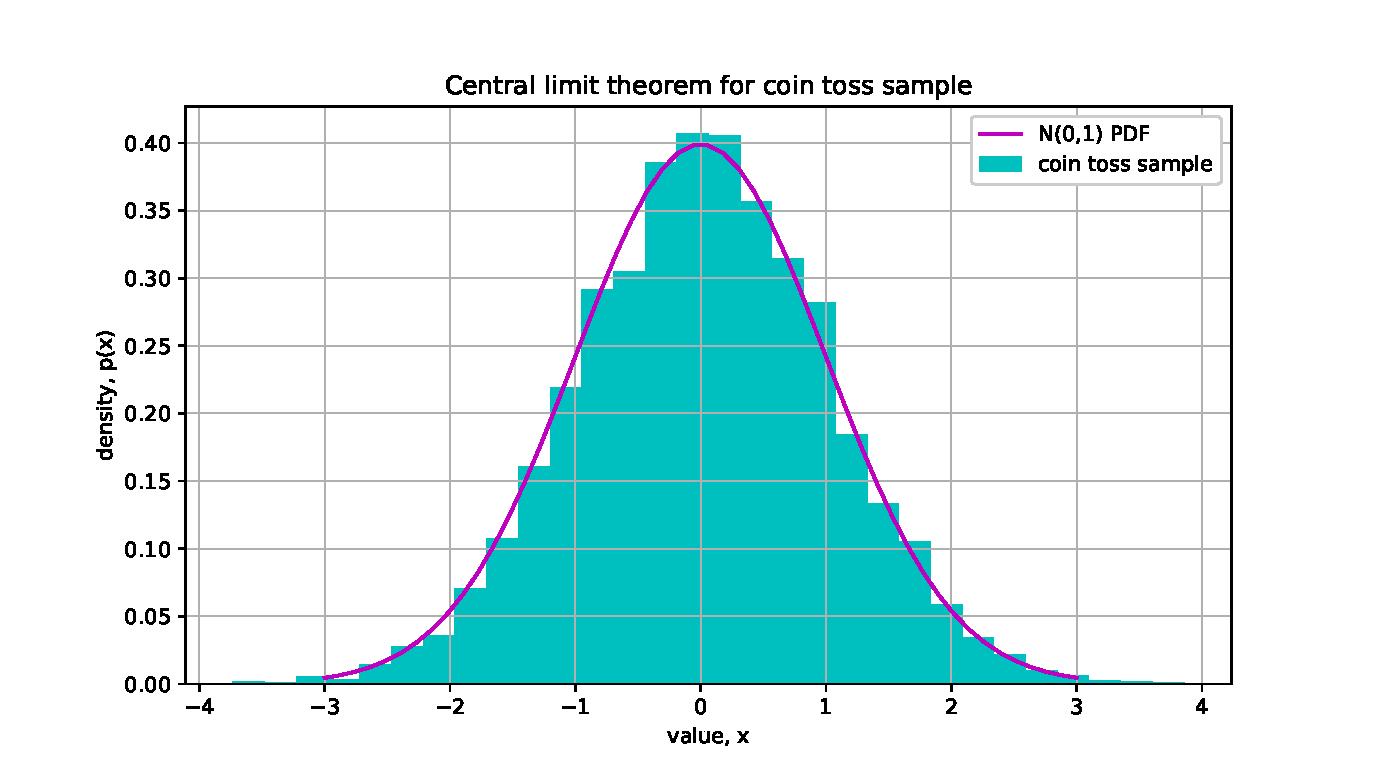
\includegraphics[width=0.9\linewidth]{coin-toss-clt.eps}
    \caption{ЦПТ для $Y_n=S_n/\sqrt{n}, n=1000$ на выборке размера $N=10^4$.}
    \label{fig:coin-toss-clt}
\end{figure}

\section{Задание 2}

\subsection{Условие}

\begin{enumerate}
\item Построить датчик сингулярного распределения, имеющий в качестве функции распределения канторову лестницу. С помощью критерия Колмогорова убедиться в корректности работы датчика.
\item Для канторовых случайных величин с помощью критерия Смирнова проверить свойство симметричности относительно $\frac{1}{2}$ ($X$ и $1 - X$ распределены одинаково) и свойство самоподобия относительно деления на $3$ (условное распределение $Y$ при условии $Y \in [0, 1/3]$ совпадает с распределением $\frac{Y}{3}$).
\item Рассчитать значения математического ожидания и дисперсии для данного распределения. Сравнить теоретические значения с эмпирическими (для различных объемов выборок), проиллюстрировать сходимость эмпирических значений
к теоретическим.
\end{enumerate}

\subsection{Генератор канторового распределения}

Канторовская лестница задаётся на множестве Кантора (которое имеет нулевую меру Лебега) отрезка $[0,1]$, доопределяется по непрерывности в оставшихся точках. Канторовское распределение имеет функцию распределения, являющейся канторовской лестницей.

Есть два способа моделирования такого распределения:
\begin{enumerate}
\item По заданному $x\in[0,1]$. Канторовское множество состоит из тех точек, у которых нет единицы в троичной записи. Переведем $x$ в троичную запись, а затем отбросим все цифры после первой (самой левой) единицы.
\item По заданному размеру выборки $N$. Будем $N$ раз моделировать $n_{\operatorname{bits}}$ испытаний схемы Бернулли с $p=\frac{1}{2}$. Все единицы заменим на двойки, и получим троичную запись числа, в которой отсутствуют единицы.
\end{enumerate}

Значением функции распределения $F(x)$ будет являться двоичное представление числа $x$. Его можно получить, заменив все двойки в троичной записи данного числа на единицы.

Число испытаний схемы Бернулли $n=n_{\operatorname{bits}}$ можно задавать с учётом заданной погрешности $\varepsilon$. В худшем случае отбрасываются двойки в троичной записи числа.
$$
\sum_{k=n+1}^{\infty} \dfrac{2^{k}}{3^{k}} = \dfrac{(\frac{2}{3})^{n+1}}{1 - \frac{2}{3}} < \varepsilon.
\quad\Rightarrow\quad
n + 1 < \log_{\frac{2}{3}}3\varepsilon.
$$

Будем генерировать канторового распределение по заданному размеру выборки $N$ и точности $\varepsilon$.

На рисунке \ref{fig:kantor-ecdf} продемонстрировано совпадение смоделированной выборки с её эмпирической функцией распределения.

\begin{figure}[H]
    \centering
    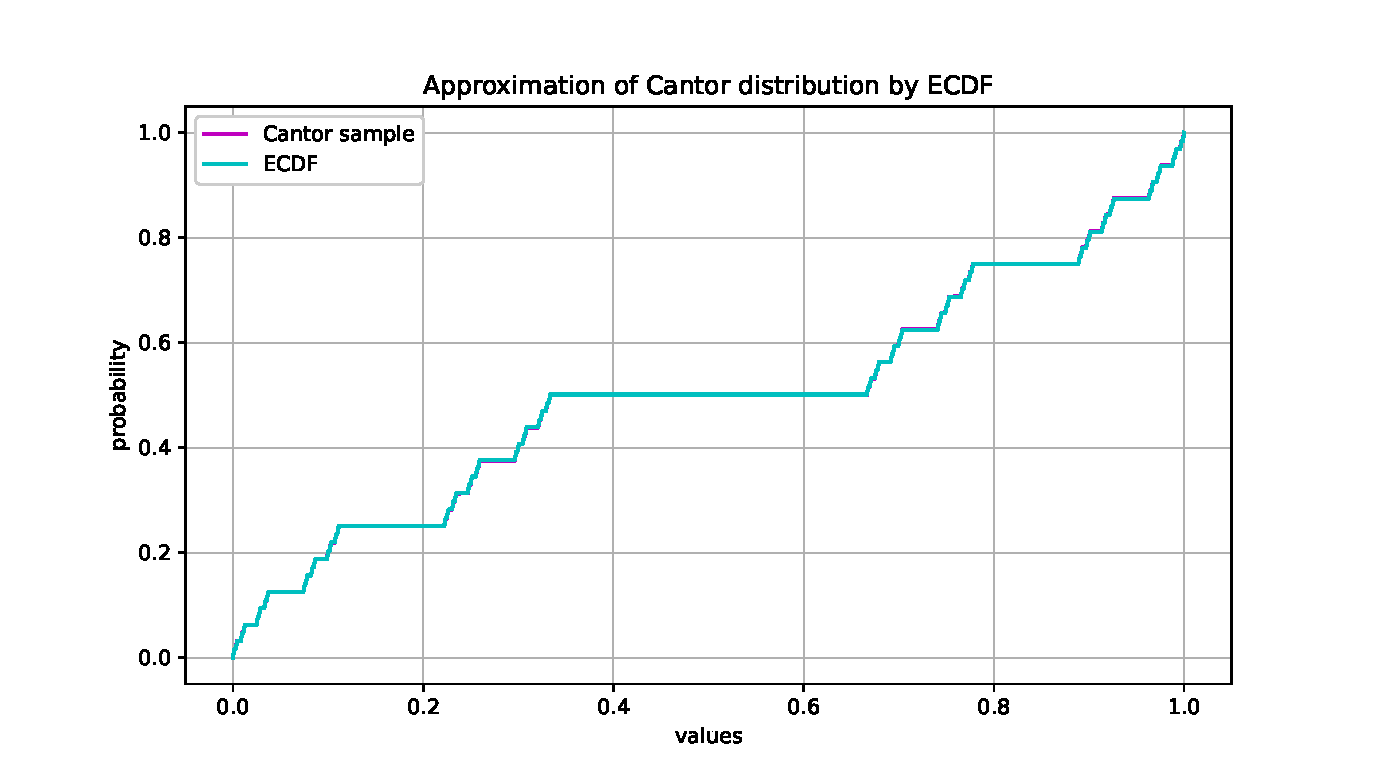
\includegraphics[width=0.9\linewidth]{kantor-ecdf.eps}
    \caption{Результат моделирования канторового распределения при $\eps =10^{-12}, (n_{\operatorname{bits}}=64),$ сравнение с эмпирической функцией распределения на выборке размера $N=10^5$.}
    \label{fig:kantor-ecdf}
\end{figure}

\begin{theorem}[Колмогоров] Пусть $X_1,X_2,\dots,X_n$ — н.о.р.с.в. с непрерывной функцией распределения $F(x)$.
Пусть $F_n(x) = \frac{1}{n}\sum_{i=1}^n \mathbb{I}\{X_{(i)}<x\}$ — эмпирическая функция распределения (ECDF).
Тогда 
$$
\forall x>0\quad \lim_{n\to\infty} \mathbb{P}({\sqrt{n}D_n < x}) = F_K(x),
$$
где $D_n=\sup\limits_{x\in\mathbb{R}}|F_n(x)-F(x)|$ — статистика Колмогорова и $F_K(\cdot)$ — функция распределения Колмогорова, которую можно выразить по формуле
$$
F_K(x) = 1 + 2 \sum_{k=1}^{+\infty}(-1)^k e^{-2k^2x^2}.
$$
\end{theorem}
\begin{proof} Приведено в \cite{shiryaev-1}. \end{proof}

Проверяем гипотезу
$$
H_0:~F(\cdot)=G(\cdot)
$$
с уровнем значимости $\alpha$, где $G=F_C(\cdot)$ — канторово распределение при помощи критерия Колмогорова.

Заметим, что $D_n$ является случайной величиной, ведь $F_n(x)$ зависит от реализации выборки.
Теорема Колмогорова утверждает, что при истинности $H_0$ выполняется $\lim\limits_{n\to\infty} D_n = 0$, $\sqrt{n}D_n \sim F_K$ при $n\to\infty$.

Будем принимать $H_0$, если $1-F_K(\sqrt{n}D_n) > \alpha$.

При проверке истинности гипотезы при помощи критерия Колмогорова $1000$ раз с уровнем значимости $\alpha=0.05$ для смоделированных датчиком канторового распределения выборок размера $N=2000$ с погрешностью $\varepsilon=10^{-6}$ нулевая гипотеза была принята в $95.6\%$ случаев.

\subsection{Свойства канторового распределения}

\begin{theorem}[Смирнов] Пусть $X_1,X_2,\dots,X_n$ и $Y_1,Y_2,\dots,Y_m$, $m\leqslant n$ две независимые выборки, подчиняющиеся одному закону распределения $F(\cdot)\in C$, и $F_n(x),G_m(y)$ — соответствующие эмпирические функции распределения. Тогда
$$
\forall x\geqslant 0\quad \lim\limits_{n,m\to\infty}\mathbb{P}\left( \sqrt{\dfrac{nm}{n+m}}D_{nm} < x \right) = F_K(x),
$$
где $D_{nm} = \sup\limits_{x\in\mathbb{R}}|F_n(x) - G_m(x)|$ — статистика Смирнова и $F_K(\cdot)$ — функция распределения Колмогорова.
\end{theorem}
\begin{proof} Приведено в \cite{shiryaev-1}. \end{proof}

Проверяем гипотезу $H_0$ для двух выборок $X$ и $Y$ с функциями распределения $F_X$ и $F_Y$:
$$
H_0:~ F_X(\cdot) = F_Y(\cdot) = F(\cdot)
$$
с уровнем значимости $\alpha$ при помощи критерия Смирнова.

Теорема Смирнова утверждает, что при истинности гипотезы $H_0$ верно $D_{nm}\to0$, $\sqrt{\frac{nm}{n+m}}D_{nm}\sim F_K$ при $n,m\to\infty$.

Будем принимать $H_0$, если $1-F_K(\sqrt{\frac{nm}{n+m}}D_n) > \alpha$.

Пусть $X$  выборка, соответствующая канторовому распределению.
\begin{enumerate}
\item Для проверки симметричности относительно $\frac{1}{2}$ выбираем $Y=1-X$.
\item Для проверки самоподобия относительно деления на 3 выбираем $\tilde{X}=\frac{X}{3}$, $Y=X$ при условии $X\in[0,\frac{1}{3}]$.
\end{enumerate}

При проверке симметричности относительно $\frac{1}{2}$ при помощи Критерия Смирнова 1000 раз с уровнем значимости $\alpha=0.05$ для выборок размера $N=1000$ с погрешностью $\eps=10^{-8}$ нулевая гипотеза была принята в $95.4\%$ случаев.

\begin{figure}[H]
    \centering
    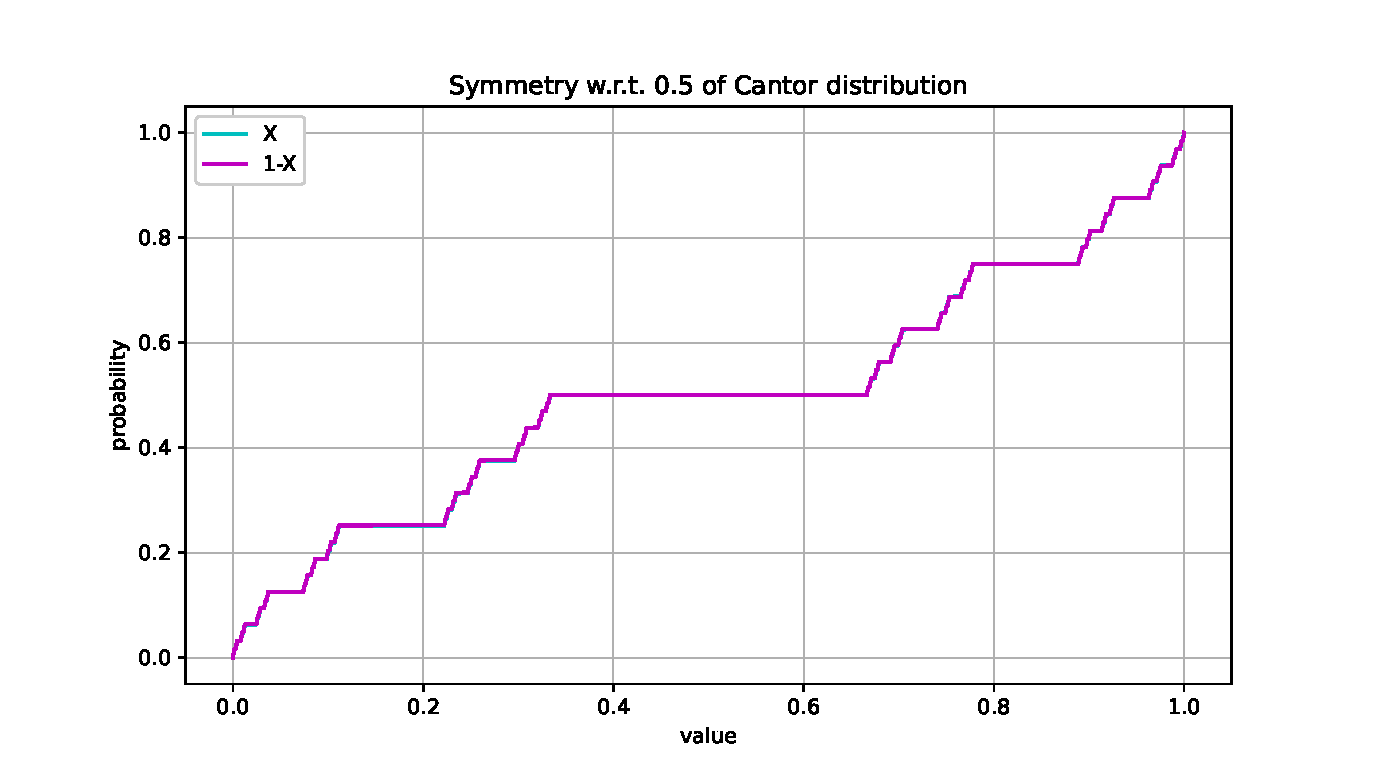
\includegraphics[width=0.9\linewidth]{kantor-symm-half.eps}
    \caption{Симметричность канторового распределения относительно $\frac{1}{2}$ при $\eps=10^{-8},N=1000$.}
    \label{fig:kantor-symm-half}
\end{figure}

При проверке симметричности относительно деления на 3 при помощи Критерия Смирнова 1000 раз с уровнем значимости $\alpha=0.05$ для выборок размера $N=10^4$ с погрешностью $\eps=10^{-12}$ нулевая гипотеза была принята в $94.0\%$ случаев.

\begin{figure}[H]
    \centering
    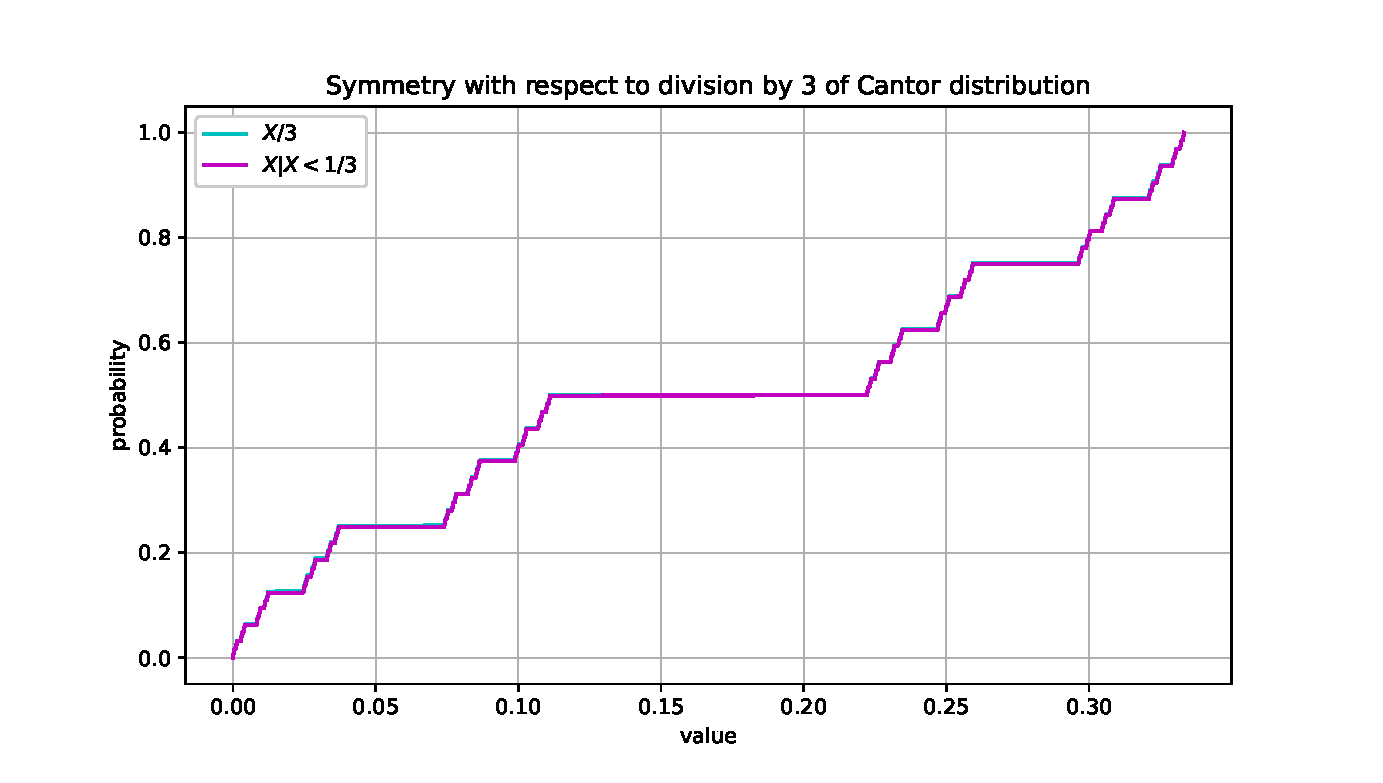
\includegraphics[width=0.9\linewidth]{kantor-symm-division.eps}
    \caption{Симметричность канторового распределения относительно деления на 3 при $\eps=10^{-12},N=10^4$.}
    \label{fig:kantor-symm-division}
\end{figure}

На рисунках \ref{fig:kantor-symm-half}, \ref{fig:kantor-symm-division} продемонстрирована симметричность относительно $\frac{1}{2}$ и деления на 3 (совпадение ECDF двух выборок на каждом рисунке).

\subsection{Численные характеристики канторового распределения}

\begin{statement}[закон полной вариации]
Пусть $X,Y$ --- случайные величины на одном вероятностном пространстве и $\mathbb{D}X<\infty$. Тогда
$$
\mathbb{D}X = \mathbb{E}[\mathbb{D}(X|Y)] + \mathbb{D}(\mathbb{E}[X|Y]).
$$
\end{statement}
\begin{proof}
По телескопическому свойству условного математического ожидания и определению дисперсии имеем
$$
\begin{aligned}
\mathbb{D}X &= \mathbb{E}X^2 - (\mathbb{E}X)^2 = \mathbb{E}[\mathbb{E}[X^2|Y]] - (\mathbb{E}[\mathbb{E}[X|Y]])^2 = \\
&= \mathbb{E}[\mathbb{D}(X|Y) + (\mathbb{E}[X|Y])^2] - (\mathbb{E}[\mathbb{E}[X|Y]])^2 = \\
&= \mathbb{E}[\mathbb{D}(X|Y)] + \underbrace{(\mathbb{E}[(\mathbb{E}[X|Y])^2] - (\mathbb{E}[\mathbb{E}[X|Y]])^2)}_{=\mathbb{D}(\mathbb{E}[X~|~Y])}=\\
&= \mathbb{E}[\mathbb{D}(X|Y)] + \mathbb{D}(\mathbb{E}[X|Y]).
\end{aligned}
$$.
Свойства условного математического ожидания и их доказательство можно найти в \cite{shiryaev-1}.
\end{proof}

\begin{itemize}
\item Математическое ожидание $X\sim F_C$, $F_C$ - канторово, равно $\frac{1}{2}$:
$$
\begin{aligned}
\mathbb{E}X &= \{X\stackrel{d}{=}1-X \} = \mathbb{E}[1-X] \\ 
\Rightarrow~\mathbb{E}X &= 1 - \mathbb{E}X \\ 
\Rightarrow~\mathbb{E}X &= \frac{1}{2}.
\end{aligned}
$$
\item Дисперсия $X\sim F_C$ равна $\frac{1}{8}$:
$$
\begin{aligned}
Y &\stackrel{def}{=} \mathbb{I}\left\{ X\in\left[\frac{2}{3},1\right]\right\}. \\
\mathbb{D}X &= \mathbb{E}[\mathbb{D}(X~|~Y)] + \mathbb{D}(\mathbb{E}[X~|~Y]). \\
\mathbb{E}[\mathbb{D}(X~|~Y)] &= \frac{1}{9}\mathbb{D}X \text{ (из свойства самоподобия)}. \\
\mathbb{E}[X~|~Y] &= \begin{cases}\begin{array}{cc}
\frac{1}{6},~ \text{с вероятностью } \frac{1}{2}, \\
\frac{1}{2},~ \text{с вероятностью } \frac{1}{2}.
\end{array}\end{cases}\text{ (из свойства симметричности)} \\
\mathbb{D}X &= \frac{1}{9}\mathbb{D}X + \frac{1}{9} \\
\Rightarrow~ \mathbb{D}X &= \frac{1}{8}.
\end{aligned}
$$
\end{itemize}

На рисунке \ref{fig:kantor-moments} продемонстрирована зависимость математического ожидания и дисперсии от размера выборки канторового распределения, сходимость эмпирических значений к теоретическим на логарифмической шкале. С увеличением размера выборки разброс относительно теоретических значений уменьшается.

\begin{figure}[H]
    \centering
    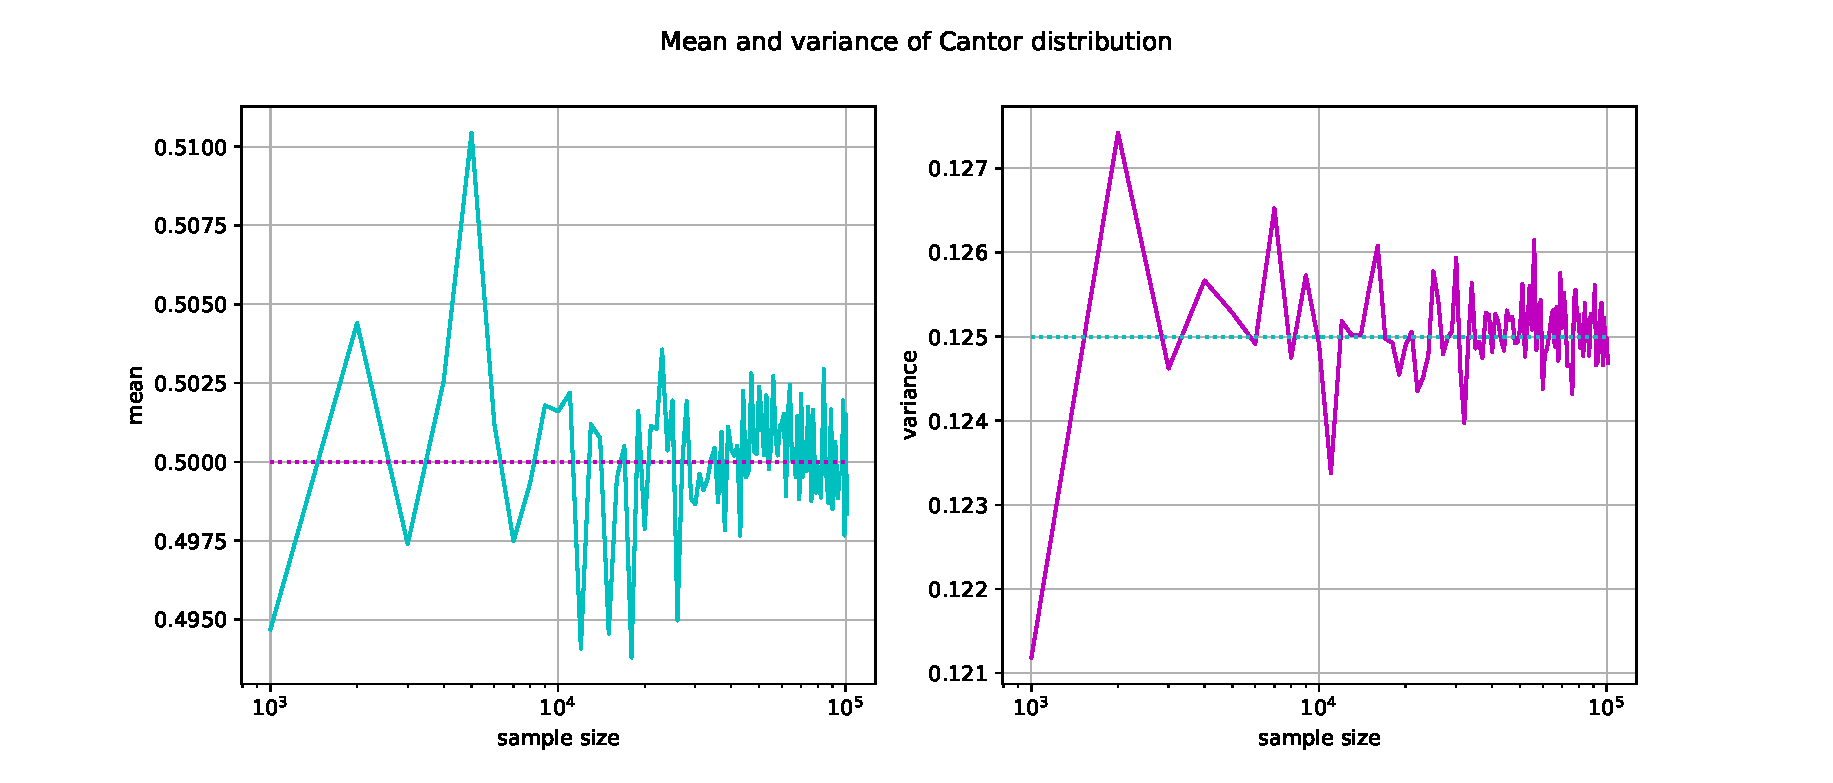
\includegraphics[width=1\linewidth]{kantor-moments.eps}
    \caption{Зависимость математического ожидания и дисперсии от выборки канторового распределения на сетке $N\in[10^3,10^5]$ с шагом $h=10^3$.}
    \label{fig:kantor-moments}
\end{figure}

\section{Задание 3}

\subsection{Условие}

\begin{enumerate}
\item Построить датчик экспоненциального распределения. Проверить для данного
распределения свойство остутствия памяти.

\item Пусть $X_1,X_2,\dots,X_n$ --- независимые экспоненциально распределенные случайные величины с параметрами
$\lambda_1,\lambda_2,\dots,\lambda_n$. Найти распределение случайной величины $Y=\min\{X_1,X_2,\dots,X_n\}$.

\item На основе датчика экспоненциального распределения построить датчик пуассоновского распределения.

\item Построить датчик пуассоновского распределения как предел биномиального распределения. Убедиться в корректности
построенного датчика при помощи критерия $\chi^2$ Пирсона.

\item Построить датчик стандартного нормального распределения методом моделирования случайных величин парами с переходом в полярные координаты 
(преобразование Бокса-Мюллера). Проверить при помощи t-критерия Стьюдента равенство математических ожиданий, а при помощи критерия Фишера — равенство дисперсий.
\end{enumerate}

\subsection{Генератор экспоненциального распределения}

\begin{definition}
Экспоненциальное распределение --- абсолютно непрерывное распределение с плотностью $\lambda e^{-\lambda x},~\lambda>0,x\geqslant 0$.
\end{definition}

Рассмотрим $\lambda > 0$. Будем генерировать случайную величину
$$
\xi = -\frac{1}{\lambda}\ln\nu,\quad \nu\sim\mathrm{U}[0,1].
$$
Она имеет экспоненциальное распределение $\mathrm{Exp}(\lambda)$, ведь
$$
\mathbb{P}(\xi < x) = \mathbb{P}(-\frac{1}{\lambda}\ln\nu < x) = \mathbb{P}(\nu > e^{-\lambda x}) = 1 - e^{-\lambda x}.
$$

\begin{figure}[H]
    \centering
    \includegraphics[width=0.9\linewidth]{images/expo.eps}
    \caption{Корректность работы датчика на примере выборки из распределения $\Exp(0.5)$ размера $N=10^5$.}
    \label{fig:expo}
\end{figure}

\begin{statement}
Случайная величина $\xi\sim\Exp(\lambda),\lambda>0$ обладает свойством отсутствия памяти:
$$
\p(\xi > t+\Delta t ~|~ \xi \geqslant t) = \p(\xi > \Delta t),\quad \forall t,\Delta t \geqslant 0.
$$
\begin{proof}
\begin{gather*}
\p(\xi > t+\Delta t ~|~ \xi \geqslant t) = \dfrac{\p(\xi > t+\Delta t)}{\p(\xi \geqslant t)}.
\end{gather*}
Отдельно вычислим
\begin{gather*}
\p(\xi > x) = 1 - \p(\xi \leqslant x) = 1 - (1 - e^{-\lambda x}) = e^{-\lambda x}.
\end{gather*}
Тогда
$$
\p(\xi > t+\Delta t ~|~ \xi \geqslant t) = \dfrac{e^{-\lambda(t+\Delta t)}}{e^{-\lambda t}} = e^{-\lambda\Delta t} = \p(\xi > \Delta t).
$$
\end{proof}
\end{statement}

На рисунке \ref{fig:expo-memo} аналогично пункту \ref{ss:geom} численно показали отсутствие памяти экспоненциального распределения.

\begin{figure}[H]
    \centering
    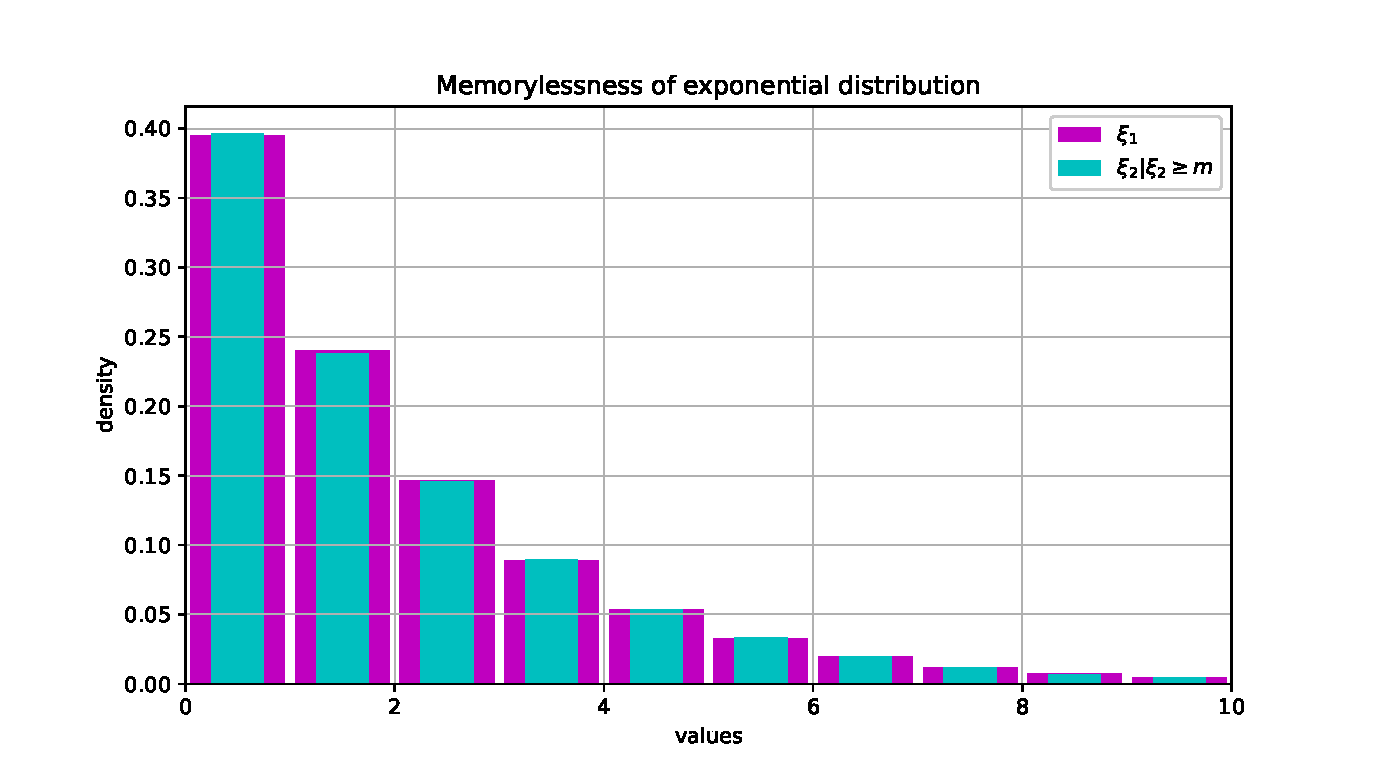
\includegraphics[width=0.9\linewidth]{images/expo-memo.eps}
    \caption{Свойство отсутствия памяти для $\Exp(0.5), \Delta t=5$ для выборок размера $N=10^6$.}
    \label{fig:expo-memo}
\end{figure}

\subsection{\texorpdfstring{Распределение $Y=\min\{X_1,X_2,\dots,X_n\}$}{Распределение минимума экспоненциальных величин}}

Положим
$$
X_k \sim \mathrm{Exp}(\lambda_k),~ k\in\overline{1,n} \text{ --- н.о.р.с.в.}
$$

Генератор строим из следующих соображений.
$$
\begin{aligned}
\mathbb{P}(Y < x) &= 1 - \mathbb{P}(\min\{X_1,X_2,\dots,X_n\} \geqslant x) = \\
&= 1 - \mathbb{P}(X_1 \geqslant x, X_2 \geqslant x, \dots, X_n \geqslant x) = \{\text{независимость}\} = \\
&= 1 - \prod_{k=1}^{n}\mathbb{P}(X_k \geqslant x) = 1 - \prod_{k=1}^{n}(1 - \mathbb{P}(X_k < x)) = \\
&= 1 - \prod_{k=1}^{n}e^{-\lambda_kx} = 1 - e^{-(\lambda_1+\lambda_2+\dots+\lambda_n)x}.
\end{aligned}
$$
Получили, что $Y\sim\mathrm{Exp}(\sum_{k=1}^n\lambda_k)$.

На рисунке \ref{fig:min-expo.eps} продемонстрировано совпадение ECDF для выборки из $Y$ и выборки из $\Exp(\sum_{k=1}^n\lambda_k)$.

\begin{figure}[H]
    \centering
    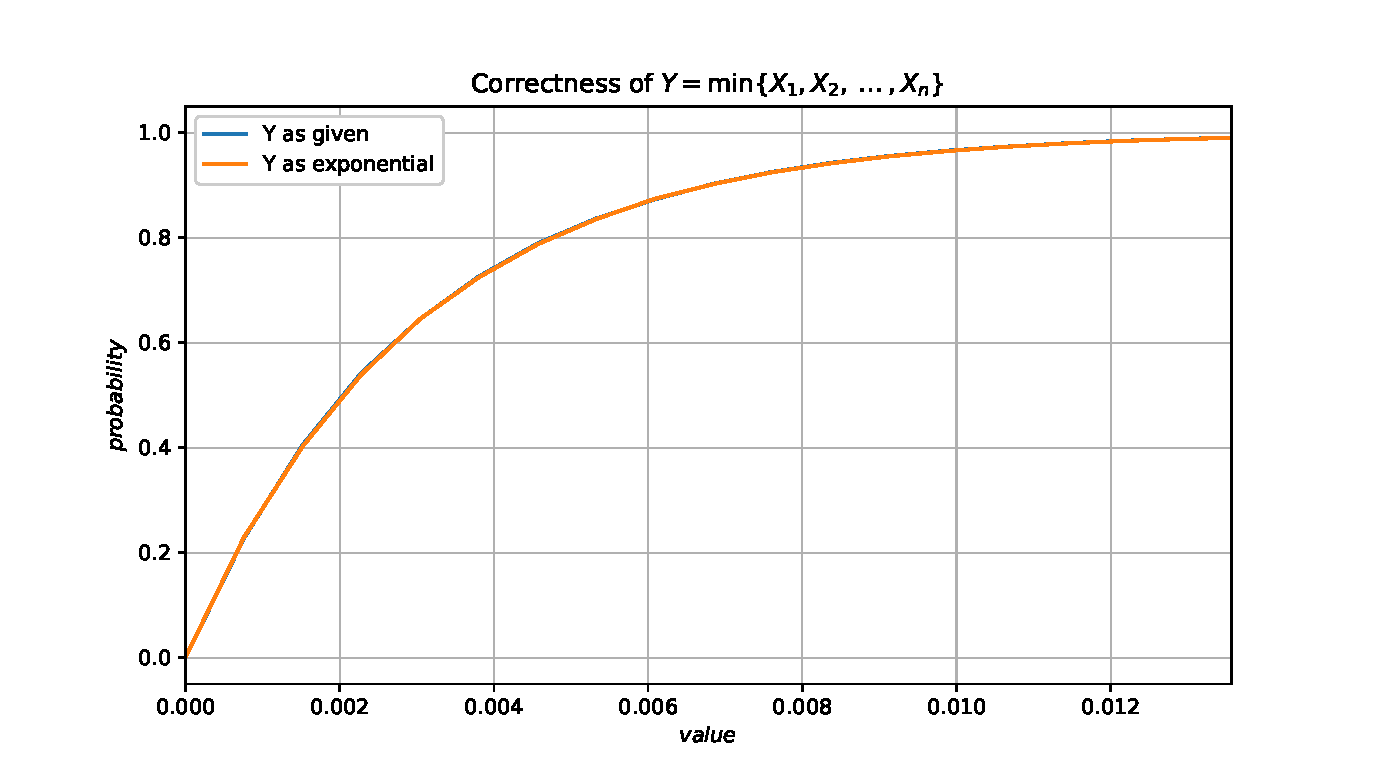
\includegraphics[width=0.9\linewidth]{images/min-expo.eps}
    \caption{Корректность работы датчика для выборки из $Y$ размера $N=10^5$, вектор $\hat\lambda$ --- выборка равномерного распределения на $[0,7]$ размера $n=100$}
    \label{fig:min-expo.eps}
\end{figure}

\subsection{Генератор пуассоновского распределения (через г-р экспоненциального р-я)}

\begin{definition}
Случайная величина $\xi\in\mathbb{N}_0$ имеет распределение Пуассона с параметром $\lambda>0$ $(\Pois(\lambda))$, если
$$
\p(\xi = k) = e^{-\lambda}\dfrac{1}{k!}\lambda^k,\quad \forall k\in\mathbb{N}_0.
$$
\end{definition}

Воспользуемся следующей теоремой.

\begin{theorem} Пусть $X_1,X_2,\dots,X_n$ - н.о.р.с.в., $X_i\sim\mathrm{Exp}(\lambda),\lambda>0$. \
Положим $Y$ --- наименьшее неотрицательное целое число такое, что
$$
\sum_{k=1}^{Y+1}X_i > 1.
$$
Тогда $Y\sim\mathrm{Pois}(\lambda)$.
\end{theorem}
\begin{proof}
Приведено в \cite{devroye}, с.501
\end{proof}

\begin{figure}[H]
    \centering
    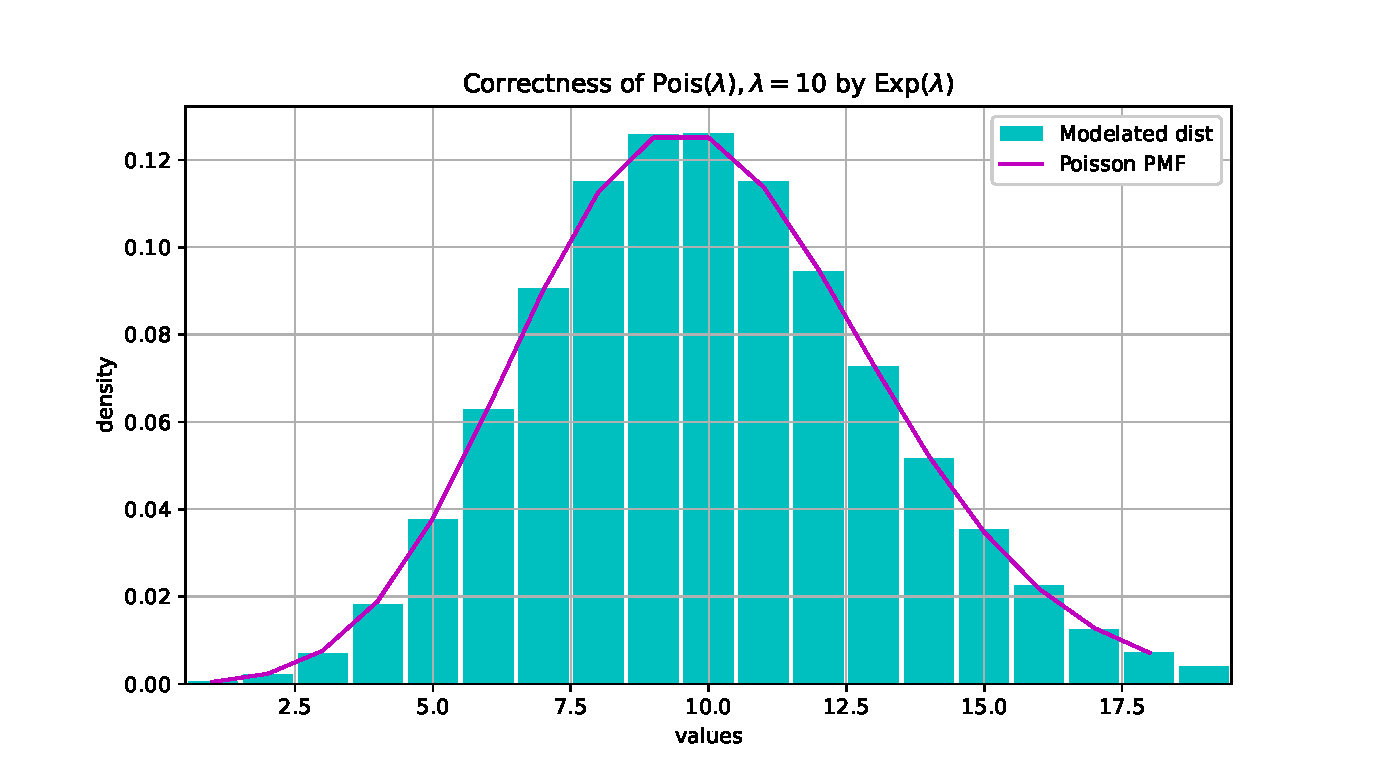
\includegraphics[width=0.9\linewidth]{images/poisson-expo.eps}
    \caption{Корректность работы датчика $\Pois(\lambda)$ при помощи датчика $\Exp(\lambda)$ при $\lambda=10,N=10^5$.}
    \label{fig:poisson-expo}
\end{figure}

\subsection{Генератор пуассоновского распределения (через г-р биномиального р-я)}

\begin{definition}
Пусть $Y_0,Y_1,\dots,Y_n$ --- независимые стандартно нормально распределенные случайные величины: $Y_i\sim\mathcal{N}(0,1),i=\overline{0,n}$. Тогда распределение случайной величины $\chi^2$:
$$
\chi^2 = Y_0^2 + Y_1^2 + \dots + Y_n^2
$$
называется распределением $\chi^2$ (хи-квадрат) с $n$ степенями свободы: $\chi^2\sim\chi^2(n)$.
\end{definition}

\begin{theorem}[Пуассон]
Пусть есть последовательность биномиально распределенных случайных величин $X_n\sim\mathrm{Bin}(n, p_n)$ такая, что
\begin{enumerate}
\item $n\to\infty$.
\item $np_n\to\lambda,~n\to\infty$.
\end{enumerate}
Тогда $\lim\limits_{n\to\infty}\mathbb{P}(X_n = m) = \dfrac{\lambda^m}{m!}e^{-\lambda}$.
\end{theorem}
\begin{proof}
Приведено в \cite{shiryaev-1}, Гл. I, §6, п.4.
\end{proof}

\begin{figure}[H]
    \centering
    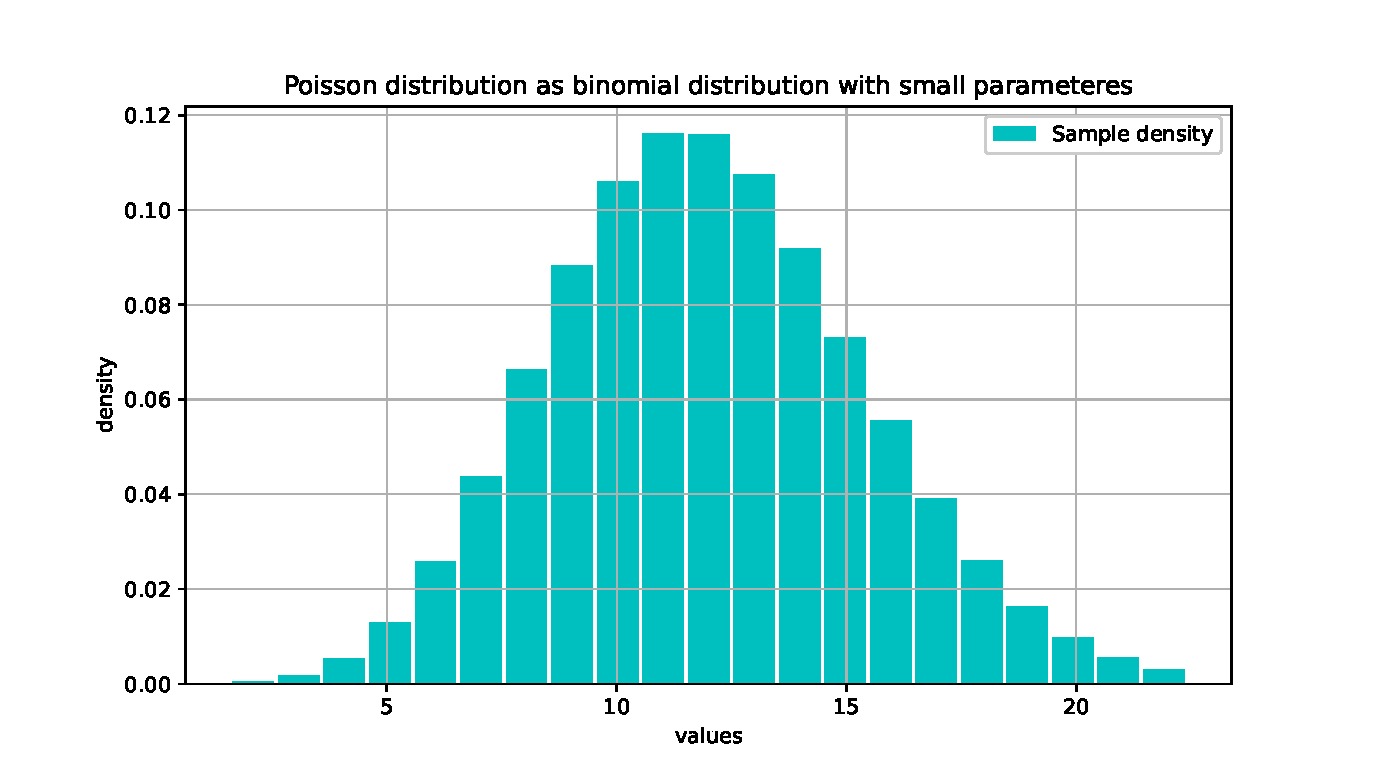
\includegraphics[width=0.9\linewidth]{images/poisson-bin.eps}
    \caption{Корректность работы датчика $\Pois(\lambda)$ при помощи датчика $\Bin(n,\lambda/n)$ при $n=10^4,\lambda=12,N=10^6$.}
    \label{fig:poisson-bin}
\end{figure}

Проверяем гипотезу о виде функции распределения $X$ при помощи критерия $\chi^2$ Пирсона:
$$
H_0:~ F_X(\cdot) = F_{\operatorname{Pois}}(\cdot)
$$
с уровнем значимости $\alpha$, где $F_{\operatorname{Pois}}(\cdot)$ - функция распределения $\mathrm{Pois}(10)$.

Выберем разбиение $T$ размера $m=15$ области определения распределения ($\mathbb{N}_0$):
$$
T = \bigcup_{k=1}^{15} T_k,\quad
T_1 = \{0,1,2,3,4\},\quad T_k=\{k+3\},k=\overline{2,14},\quad
T_{15}=\{k\geqslant18\}.
$$
Вычисляем теоретические вероятности $p_k=\mathbb{P}(X \in T_k)$ при условии истинности $H_0$.
Вычисляем $l_k$ - число попаданий значений выборки $X$ в множество $T_k$.

Согласно критерию $\chi^2$ Пирсона при истинности гипотезы $H_0$ статистика $\chi^2$:
$$
\chi^2 = \sum^{m}_{k=1} \dfrac{(l_k - np_k)^2}{np_k} = \sum^{m}_{k=1}\dfrac{n}{p_k}\left( \dfrac{l_k}{n} - p_k \right)^2
$$
имеет распределение $\chi^2_{m-1}$.

Будем принимать гипотезу, если $1-F_{\chi^2_{m-1}}(\chi^2) > \alpha$.

При проверке истинности гипотезы о виде распределения при помощи критерия $\chi^2$ Пирсона для выборки размера $N=10^4$ пуассоновского распределения, полученную как биномиальное распределение с малым параметром, в количестве 250 раз с уровнем значимости $\alpha=0.05$ гипотеза $H_0$ была принята в $95.6\%$ случаев.

\subsection{Генератор стандартного нормального распределения (преобразование Бокса-Мюллера)}

Существует эффиктивный способ моделирования пары независимых нормально распределенных случайных величин. Он основан на следующей теореме.

\begin{theorem}[преобразование Бокса-Мюллера]
Пусть $\xi_1,\xi_2$ - независимые стандартно нормально распределенные случайные величины.
Тогда их можно представить в виде
$$
\begin{cases}
\xi_1 = \sqrt{\omega}\cos\nu,\\
\xi_2 = \sqrt{\omega}\sin\nu.
\end{cases}
$$
где $\nu\sim\mathrm{U}[0,2\pi], \omega\sim\mathrm{Exp}(\frac{1}{2})$ - независимые.
\end{theorem}
\begin{proof}
Покажем, что совместные плотности векторов
$$
(\xi_1,\xi_2), (\sqrt{\omega}\cos\nu, \sqrt{\omega}\sin\nu)
$$ 
совпадают.
Для этого достаточно перейти к полярным координатам под знаком интеграла:
$$
\begin{aligned}
\mathbb{P}(X_1<x, X_2<y) &= \int_{-\infty}^{x}\int_{+\infty}^{y} \dfrac{1}{2\pi}e^{-\frac{x_1^2+x_2^2}{2}}dx_2dx_1 = \\
&= \biggl\vert \begin{array}{c}
x_1 = r\cos\alpha, \\ 
x_2 = r\sin\alpha.
\end{array} \biggr\vert = \iint\limits_{\begin{array}{c}r\cos\alpha<x\\ r\sin\alpha<y\end{array}} \dfrac{1}{2\pi}e^{-\frac{r^2}{2}}rdrd\alpha = \\
&= \{ \omega = r^2, d\omega = 2rdr \} = \\
&= \iint\limits_{\begin{array}{c}\sqrt{\omega}\cos\alpha<x\\ \sqrt{\omega}\sin\alpha<y\end{array}} \dfrac{1}{2\pi}e^{-\frac{\omega}{2}}\frac{1}{2}d\omega d\alpha = \mathbb{P}(\xi_1 < x, \xi_2 < y).
\end{aligned}
$$
\end{proof}

На рисунке \ref{fig:norm-expo} продемонстрирована корректность работы датчика, основанном на преобразование Бокса-Мюллера, для моделирования выборки из стандартного нормального распределения размера $N=10^6$.

\begin{figure}[H]
    \centering
    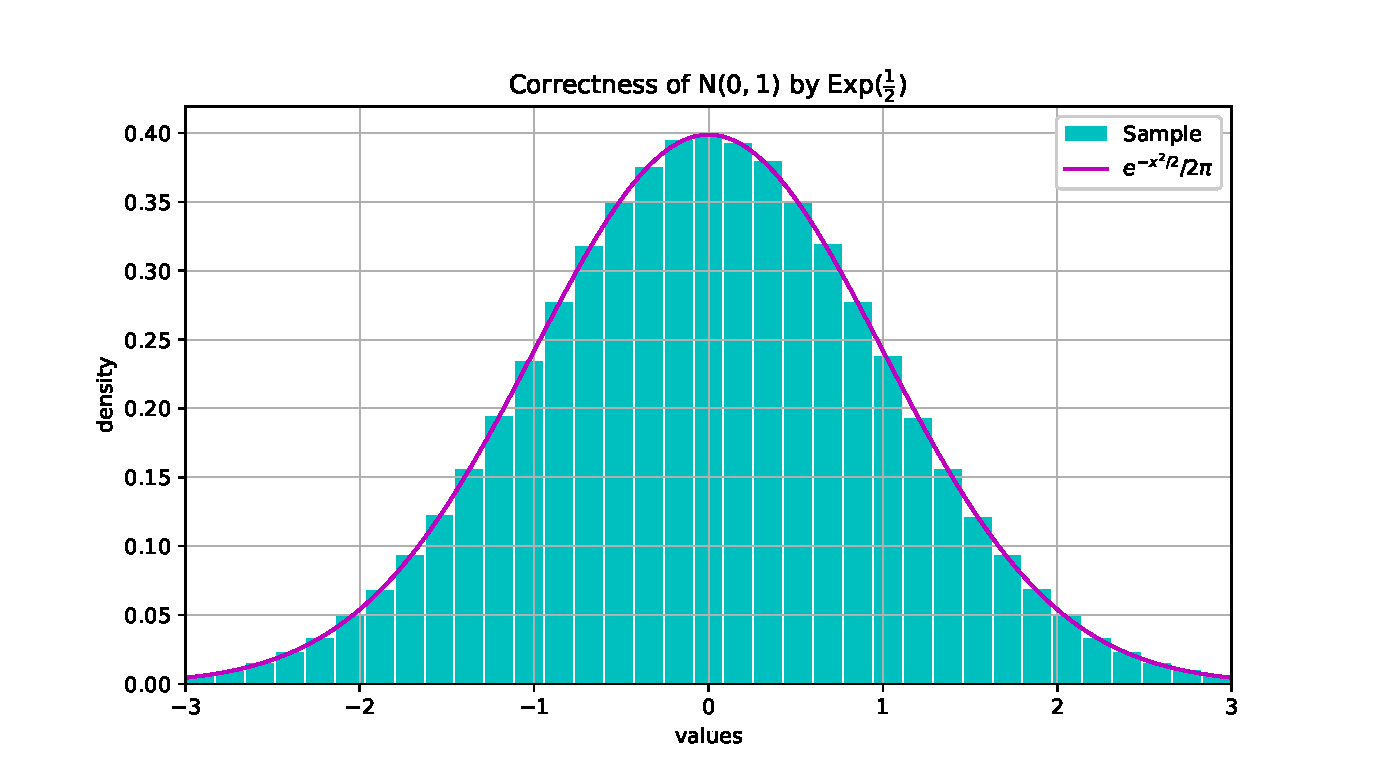
\includegraphics[width=0.9\linewidth]{images/norm-expo.eps}
    \caption{Корректность работы датчика стандартного нормального распределения через датчик экспоненциального распределения для выборки $N=10^6$.}
    \label{fig:norm-expo}
\end{figure}

\begin{definition}
Пусть $Y_0,Y_1,\dots,Y_n$ --- независимые стандартные нормально распределенные случайные величины: $Y_i\sim\mathcal{N}(0,1),i=\overline{0,n}$. Тогда распределение случайной величины $t$:
$$
t = \dfrac{Y_0}{\sqrt{\frac{1}{n}\sum^n_1Y_i^2}}
$$
называется распределением Стьюдента с $n$ степенями свободы: $t\sim \mathrm{t}(n)$.
\end{definition}

\begin{statement}[Стьюдент]
Пусть $X_1,X_2,\dots,X_n$ - независимые случайные величины такие, что $X_i\sim\mathrm{N}(\mu,\sigma^2), i=\overline{1,n}$.
Положим $\overline{X}$ - выборочное среднее, $S^2$ - несмещенная выборочная дисперсия. Тогда
$$
T=\dfrac{\overline{X}-\mu}{S/\sqrt{n}}\sim \mathrm{t}(n-1),
$$
где $\mathrm{t}(n-1)$ --- распределение Стьюдента с $(n-1)$ степенями свободы.
\end{statement}

Дополнительно проверим гипотезу о равенстве мат. ожидания конкретному значению одной нормально распределенной выборки при помощи t-критерия Стьюдента:
$$
H_0:~ \mathbb{E}X = \mu.
$$

Согласно утверждению Стьюдента при истинности гипотезы $H_0$ статистика $T$ имеет распределение $\mathrm{t}(n-1)$. \
Отметим, что критерий Стьюдента имеет двустороннюю критическую область.

Будем принимать $H_0$, если $|T| < K_\alpha = F^{-1}_{t(n-1)}(1-\alpha/2)$.

Нужные значения возьмём из таблицы: при $\alpha=0.05, n=10^4 + 1$ квантиль $K_\alpha \approx 1.9623$.

При применении описанного выше $\mathrm{t}$-критерия Стьюдента в количестве 1000 раз для выборки из $\mathcal{N}(\mu,\sigma^2),\mu = 2.5,\sigma=1.25$ размера $N=10^5$ нулевая гипотеза была принята в $95.3\%$ случаев.

\begin{definition}
Пусть $Y_1,Y_2$ --- независимые случайные величины, имеющие распределения $\chi^2(d_1),\chi^2(d_2),d_i\in\mathbb{N},i=1,2$ соответственно.
Тогда распределение случайной величины
$$
F=\dfrac{Y_1/d_1}{Y_2/d_2}
$$
называется распределением Фишера со степенями свободы $d_1,d_2$. Обозначение: $F\sim\mathrm{F}(d_1,d_2)$.
\end{definition}

Далее проверим гипотезу о равенстве дисперсий двух независимых нормально распределенных выборок при помощи критерия Фишера:
$$
H_0:~ \mathbb{D}X = \mathbb{D}Y = \sigma^2.
$$

При истинности гипотезы $H_0$ для выборок $X$ (размера $n$) и $Y$ (размера $m$) статистика
$$
D = \dfrac{S^2_X}{S^2_Y} \sim F(m-1,n-1),
$$
где $F(m-1,n-1)$ - распределение Фишера со степенями свободы $n-1$ и $m-1$. \
Отметим, что критерий Фишера также имеет двустороннюю критическую область.

Будем принимать $H_0$, если $D\in (K_{\alpha/2}, K_{1-\alpha/2})$, где $K_{\alpha/2}=F^{-1}_{F(n-1,m-1)}(\alpha/2), K_{1-\alpha/2}=F^{-1}_{F(n-1,m-1)}(1-\alpha/2)$.

При применении описанного выше критерия Фишера для двух выборок \\
$X,Y\sim\mathcal{N}(\mu,\sigma^2)$,
$\mu=2.5,\sigma=1.25$ размеров $N$ и $M$ соответственно в количестве 1000 раз с уровнем значимости $\alpha=0.05$ нулевая гипотеза была принята в $95.8\%$ случаев.

\section{Задание 4}

\subsection{Условие}

\begin{enumerate}
\item Построить датчик распределения Коши.
\item На основе датчика распределения Коши с помощью метода фон Неймана построить датчик стандартного нормального распределения. При помощи 
графика normal probability plot убедиться в корректности построенного датчика и обосновать наблюдаемую линейную зависимость.
\item Сравнить скорость моделирования стандартного нормального распределения в задании 3 и в задании 4.
\end{enumerate}

\subsection{Генератор распределения Коши}

\begin{definition}
Распределение Коши $C(x_0,\gamma)$ --- абсолютно непрерывное распределение с плотностью
$$
\dfrac{1}{\pi\gamma\left(1+(\frac{x-x_0}{\gamma})^2 \right)},
$$
где $x_0$ - параметр сдвига, $\gamma>0$ - параметр масштаба.
\end{definition}

Пусть $X\sim\mathrm{C}(x_0,\gamma)$. Тогда
$$
\begin{aligned}
F_X(x) &= \dfrac{1}{\pi}\operatorname{arctg}\left(\dfrac{x-x_0}{\gamma}\right) + \dfrac{1}{2}, \\
F_X^{-1}(x) &= x_0 + \gamma\tg\left[\pi\left(x-\dfrac{1}{2}\right)\right].
\end{aligned}
$$

Будем моделировать выборку распределения Коши метод обращения функции распределения.

На рисунке \ref{fig:cauchy-lack} продемонстрировано отсутствия математического ожидания распределения Коши.

\begin{figure}[H]
    \centering
    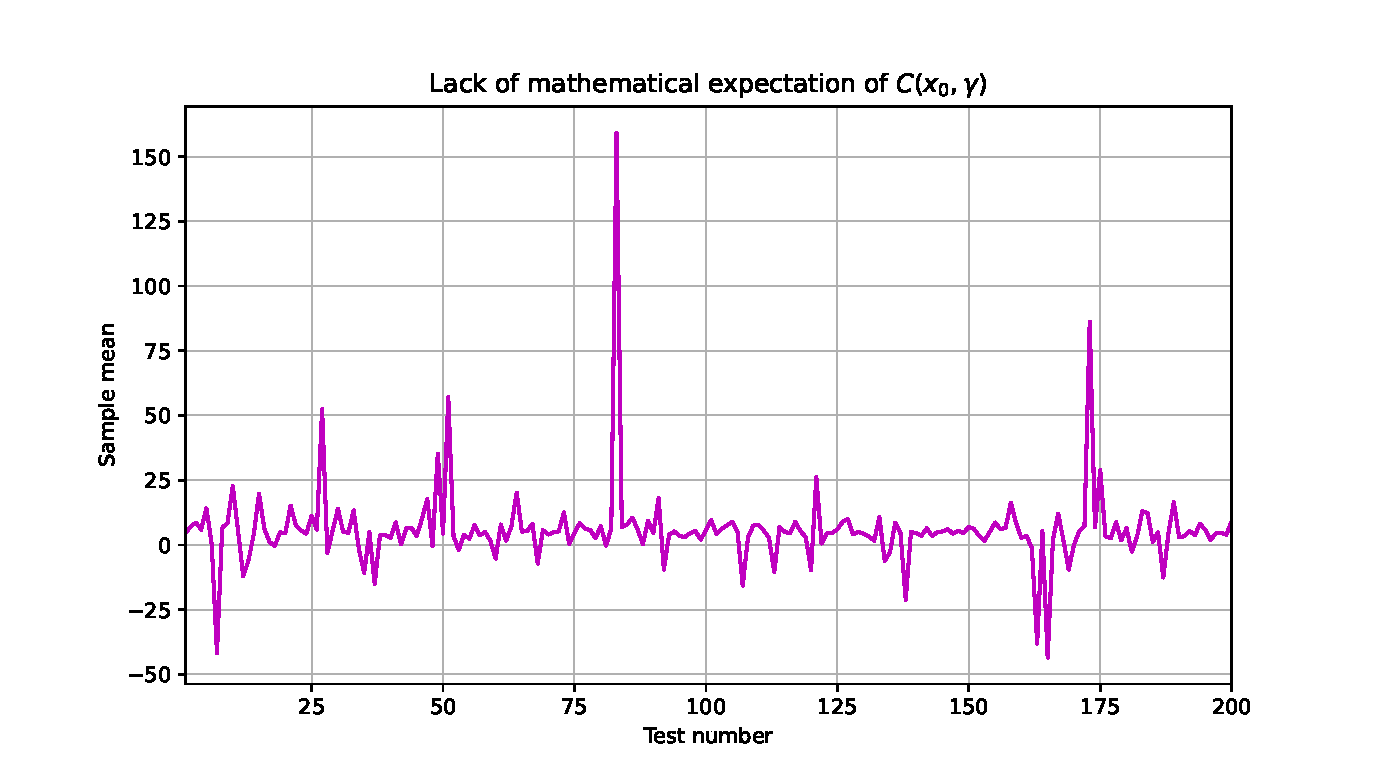
\includegraphics[width=0.9\linewidth]{images/cauchy-lack.eps}
    \caption{Мат. ожидание $C(5,2)$ в зависимости от номера запуска при $N=10^6$.}
    \label{fig:cauchy-lack}
\end{figure}

\subsection{Генератор стандартного нормального распределения (через г-р распределения Коши)}

Опишем \textit{метод элиминации фон Неймана}. \\
Ставится задача моделирования распределения с плотностью $f(x)$ со значениями в $\mathbb{R}^n.$ \\
Пусть имеются $X\sim g(x)$ и $U\sim \mathrm{U}[0,1]$ - две случайные величины, $g(x)$ принимает значения в $\mathbb{R}^n$.
Также имеется константа $c\geqslant 1$.

Можно показать, что случайный вектор $(X, cUg(X))\sim\mathrm{U}(A)$, где $A=\{(x,u)~|~x\in\mathbb{R}^n,0\leqslant u\leqslant cf(x)\}$.

Доказательство, обоснование корректности приведены в \cite{devroye}, с. 40-46.

Обоснованность алгоритма моделирования для $f(x)=\dfrac{1}{\sqrt{2\pi}}e^{-\frac{x^2}{2}}$ приведена там же, с. 46.

Функция $\texttt{scipy.stats.probplot}$ строит Q-Q plot (quantile-quantile plot). Он определяется следующим образом.
\begin{itemize}
\item По оси ординат откладывается выборка в возрастающем порядке.
\item По оси абсцисс откладываются теоретические квантили заданного распределения (в данном случае нормального).
\end{itemize}

Подсчет теоретических квантилий осуществляется при помощи преобразования Филлибена, ведь возникает проблема их вычисления для выборок малого размера.

Таким образом, чтобы проверить данные на нормальность, достаточно взглянуть на линейный порядок сортированных данных на Q-Q графике.

На рисунке \ref{fig:norm-probplot} отчётливо видна линейная зависимость, что влечёт корректность построенного датчика.

\begin{figure}[H]
    \centering
    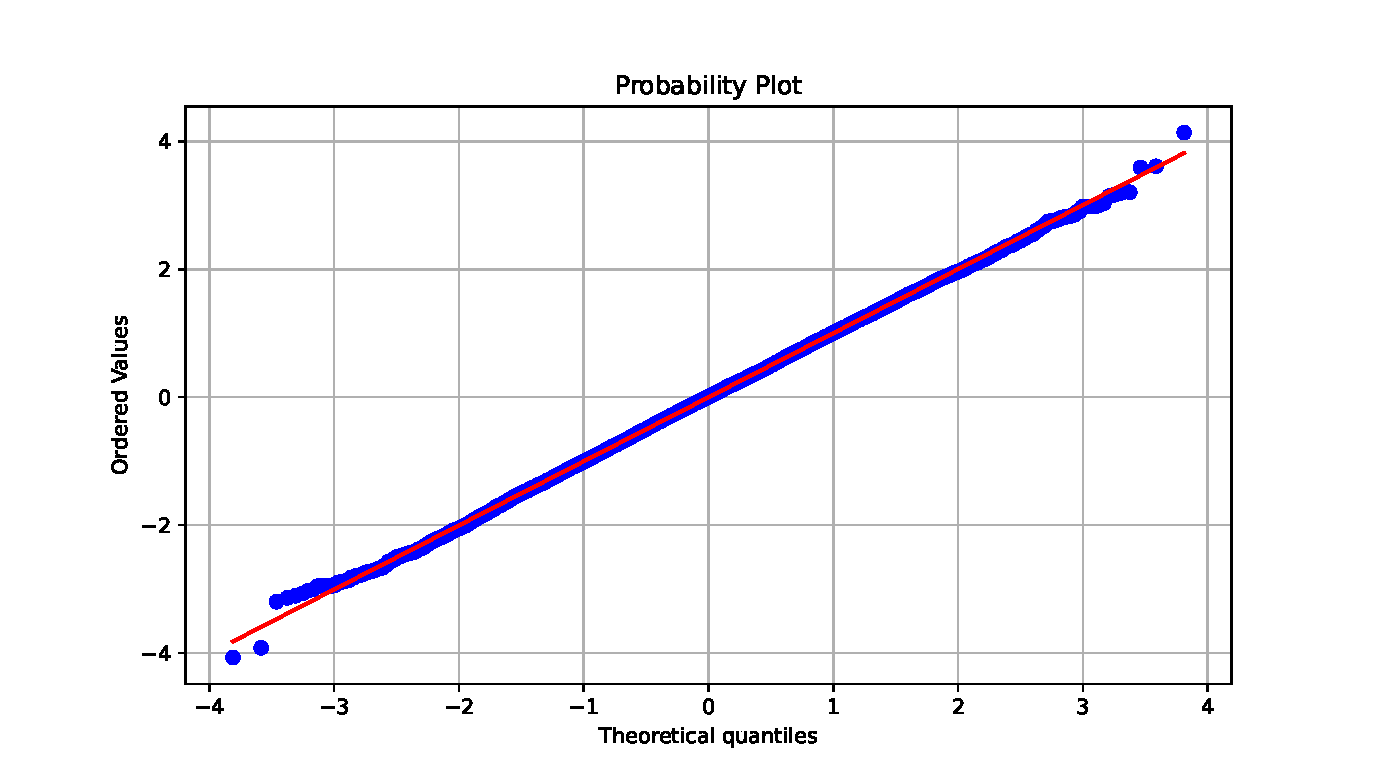
\includegraphics[width=0.9\linewidth]{images/norm-probplot.eps}
    \caption{Probability plot для выборки $\mathcal{N}(0,1)$, полученной методом элиминации, при $N=10^6$.}
    \label{fig:norm-probplot}
\end{figure}

\subsection{Сравнение скорости сходимости}

На рисунке \ref{fig:norm-times} продемонстрирована средняя скорость вычисления по 100 вычислениям в зависимости от размера выборки на логарифмической шкале.

\begin{figure}[H]
    \centering
    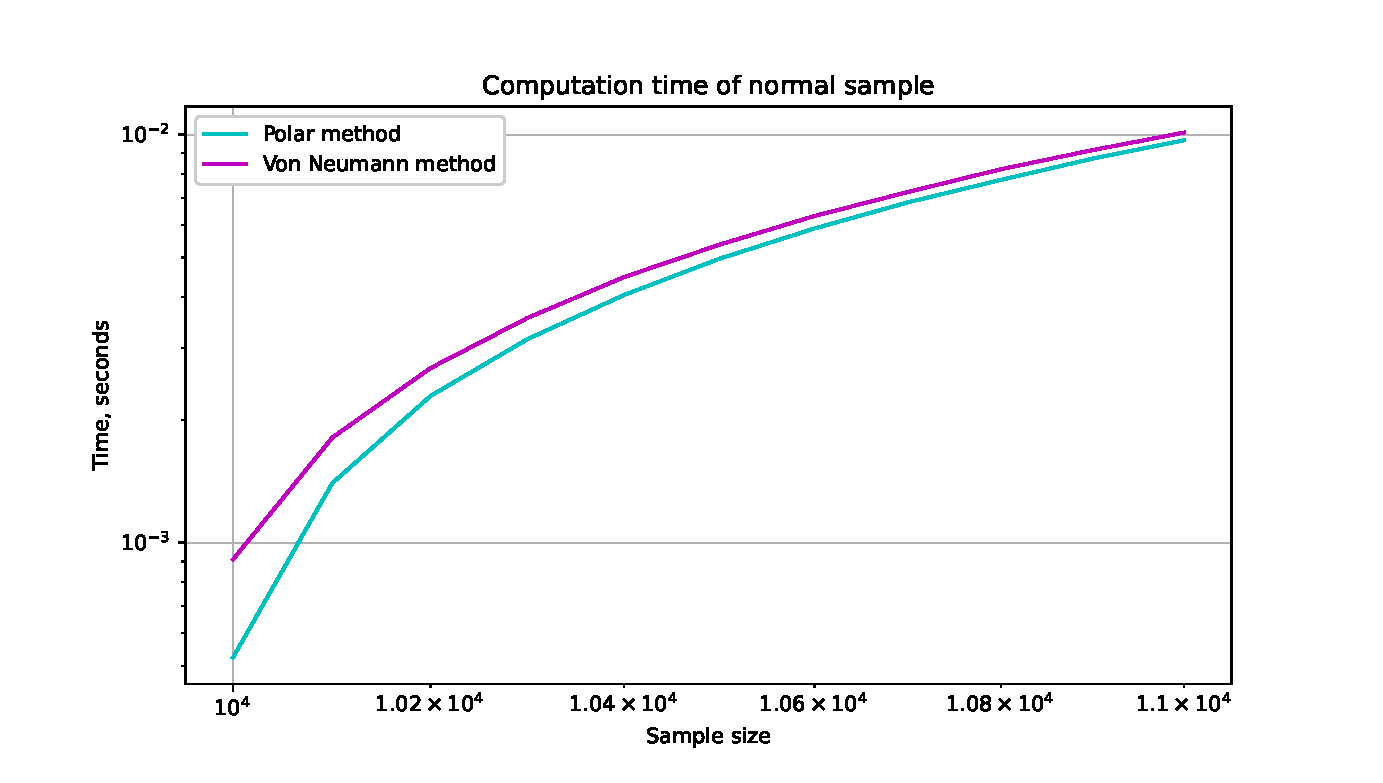
\includegraphics[width=0.9\linewidth]{images/norm-times.eps}
    \caption{Сравнение скорость моделирования выборки из стандартного нормального распределения полярным методом и методом элиминации.}
    \label{fig:norm-times}
\end{figure}

\section{Задание 5}

\subsection{Условие}

\begin{enumerate}
\item Пусть $X_i\sim \mathcal{N}(\mu,\sigma^2)$. Убедиться эмпирически в справедливости теоремы о законе больших чисел (ЗБЧ) и центральной предельной теоремы (ЦПТ): исследовать поведение суммы $S_n = \sum\limits_{i=1}^n X_i$ и эмпирического распределения величины
$$
\sqrt{n}\dfrac{S_n}{n} - a.
$$
\item Считая $\mu$, $\sigma$ неизвестными, построить доверительные интервалы для среднего и дисперсии по имеющейся выборке.
\item Пусть $X_i \sim K(a,b)$ - имеет распределение Коши с параметрами сдвига $a$ и масштаба $b$. Изучить эмпирически как ведут себя суммы $\frac{S_n}{n}$, объяснить результат и найти закон распределения данных сумм.
\end{enumerate}

\subsection{Справедливость теоремы о ЗБЧ и ЦПТ}

Сформулируем теорему о ЗБЧ в форме А.Я.Хинчина. ЦПТ сформулирована в пункте \ref{ss:coin-toss}.

\begin{theorem}[о законе больших чисел в форме А.Я.Хинчина]
Пусть $X_1,X_2,\dots$ --- последовательность н.о.р.с.в. таких, что $\mathbb{E}|X_k|<\infty,~\mathbb{E}X_1=\mu$.
Пусть $S_n = \sum_{k=1}^{n}X_k$. Тогда
$$
\forall\varepsilon>0\quad\lim_{n\to\infty}\mathbb{P}\left( \left|\dfrac{S_n}{n} - \mu\right| \geqslant \varepsilon \right) = 0.
$$
\end{theorem}
\begin{proof}
Приведено в \cite{shiryaev-1}, с.447-449.
\end{proof}

Согласно ЦПТ выполняется
$$
\sqrt{n}\left( \dfrac{S_n}{n}-\mu \right) = 
\dfrac{\frac{S_n}{n} - \mu}{\frac{1}{\sqrt{n}}} \stackrel{d}{\longrightarrow} \mathrm{N}(0,\sigma^2)
$$
На рисунке \ref{fig:norm-sum-std} это доказано эмпирически. Также, на рисунке \ref{fig:norm-sum-mean} продемонстрирована сходимость выборочного среднего к теоретическому среднему при $\mu=5, \sigma=1.5$.

\begin{figure}[H]
    \centering
    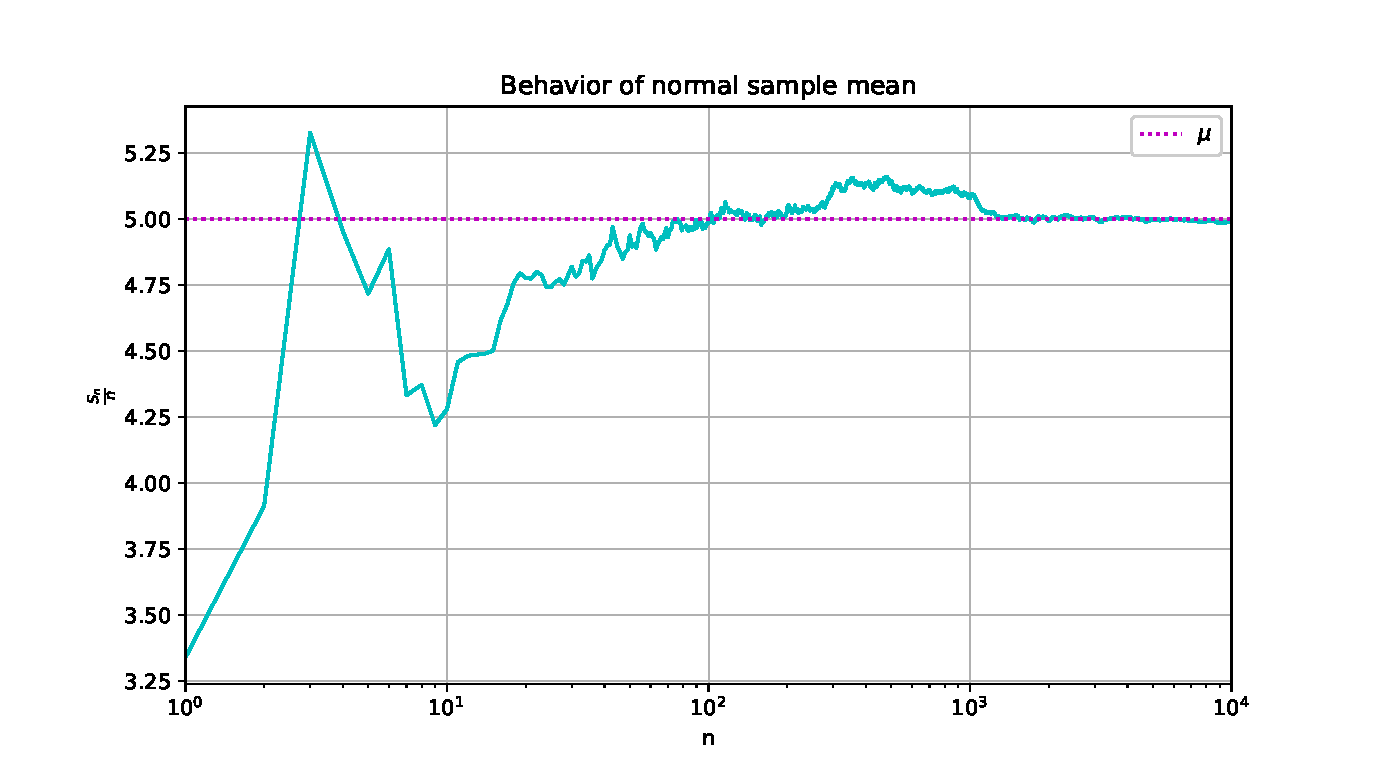
\includegraphics[width=0.85\linewidth]{images/norm-sum-mean.eps}
    \caption{Выборочное среднее суммы $S_n/n$ при $X_i\sim\mathcal{N}(5,1.5^2)$ в зависимости от размера выборки.}
    \label{fig:norm-sum-mean}
\end{figure}

\begin{figure}[H]
    \centering
    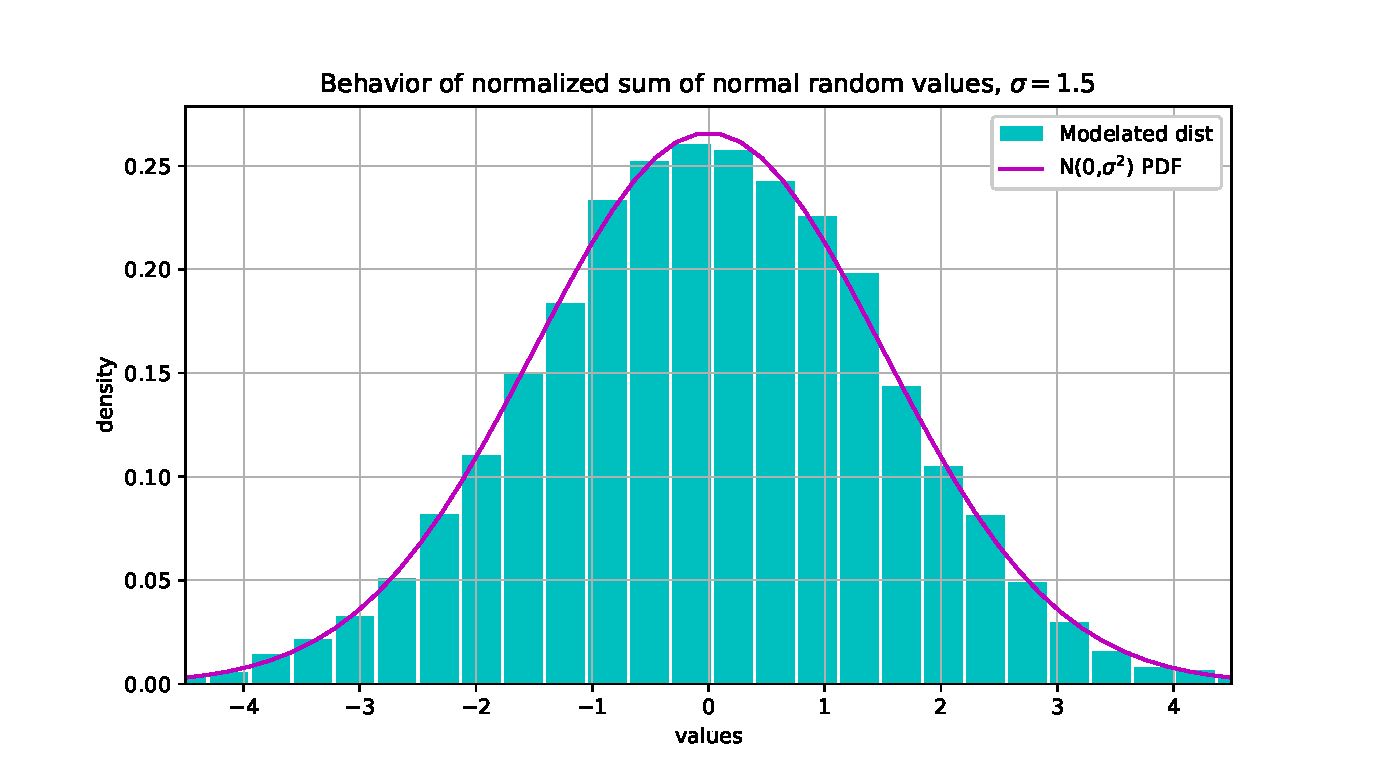
\includegraphics[width=0.85\linewidth]{images/norm-sum-std.eps}
    \caption{Распределение нормированной суммы $\sqrt{n}(\frac{S_n}{n}-\mu)$ при $\mu=5,\sigma=1.5,N=10^4$.}
    \label{fig:norm-sum-std}
\end{figure}

\subsection{Доверительные интервалы для среднего и дисперсии}

\begin{definition}
Пара статистик $T_1(X_{\theta}),T_2(X_{\theta})$ называется доверительным интервалом для параметра $\theta$ с уровнем значимости $\alpha\in[0,1]$, если
$$
\mathbb{P}(T_1(X_{\theta})\leqslant\theta\leqslant T_2(X_{\theta}) \geqslant 1-\alpha.
$$
\end{definition}

Знаем распределения следующих статистик:
$$
T = \sqrt{n}\dfrac{\overline{X} - \mu}{S} \sim t(n-1). \\
\quad D = \dfrac{\sum_{i=1}^n(\overline{X} - X_i)^2}{\sigma^2} \sim \chi^2(n-1).
$$
Здесь $\overline{X}$ - выборочное среднее, $S^2$ - несмещенная выборочная дисперсия:
$$
\overline{X} = \dfrac{\sum_{i=1}^nX_i}{n},\quad S^2 = \dfrac{\sum_{i=1}^n(\overline{X}-X_i)^2}{n-1}.
$$

Будем искать доверительные интервалы $(\gamma_1,\gamma_2)$ с уровнем значимости $\alpha$:
$$
\mathbb{P}(\gamma_1 < Y < \gamma_2) = 1-\alpha,
$$
считая $\mu,\sigma$ неизвестными. Для этого достаточно взять $\gamma_1,\gamma_2$ равными таким квантилям, что
$$
\mathbb{P}(\gamma_1 < Y < \gamma_2) = \underbrace{\mathbb{P}(Y < \gamma_2)}_{1-\frac{\alpha}{2}} - \underbrace{\mathbb{P}(Y < \gamma_1)}_{\frac{\alpha}{2}} = 1 - \alpha.
$$

Доверительный интервал для среднего $\mu$ ищем при $Y=T$.
$$
\mathbb{P}(\gamma_1 < T < \gamma_2) = \mathbb{P}\left(\gamma_1 < \sqrt{n}\dfrac{\overline{X} - \mu}{S} < \gamma_2\right) =
\mathbb{P}\left( \overline{X}-\dfrac{\gamma_2S}{\sqrt{n}} < \mu < \overline{X}-\dfrac{\gamma_1S}{\sqrt{n}} \right) = 1-\alpha.
$$
Выберем
$$
\gamma_1 = F^{-1}_{t(n-1)}\left(\frac{\alpha}{2} \right),\quad \gamma_2 = F^{-1}_{t(n-1)}\left(1-\dfrac{\alpha}{2}\right).
$$
Таким образом, $\mu\in\left(\overline{X}-\dfrac{\gamma_2S}{\sqrt{n}},\overline{X}-\dfrac{\gamma_1S}{\sqrt{n}}\right)$ с вероятностью $1-\alpha$.

Доверительный интервал для дисперсии $\sigma^2$ ищем при $Y=D$.
$$
\begin{aligned}
\mathbb{P}(\gamma_1 < D < \gamma_2) &= \mathbb{P}\left(\gamma_1 < \dfrac{\sum_{i=1}^n(\overline{X} - X_i)^2}{\sigma^2} < \gamma_2\right) = \\
&=\mathbb{P}\left( \dfrac{\sum_{i=1}^n(\overline{X} - X_i)^2}{\gamma_2} < \sigma^2 < \dfrac{\sum_{i=1}^n(\overline{X} - X_i)^2}{\gamma_1} \right) = 1-\alpha.
\end{aligned}
$$
Выберем
$$
\gamma_1 = F^{-1}_{\chi^2(n-1)}\left(\frac{\alpha}{2} \right),\quad \gamma_2 = F^{-1}_{\chi^2(n-1)}\left(1-\dfrac{\alpha}{2}\right).
$$
Таким образом, $\sigma^2\in\left(\dfrac{\sum_{i=1}^n(\overline{X} - X_i)^2}{\gamma_2}, \dfrac{\sum_{i=1}^n(\overline{X} - X_i)^2}{\gamma_1}\right)$ с вероятностью $1-\alpha$.

При проведении 1000 тестов параметр $\mu$ принадлежал доверительному интервалу с уровнем значимости $\alpha=0.05$ в $94.8\%$ случаев. Также, дисперсия $\sigma^2$ принадлежала соответствующему доверительному интервалу в $95.5\%$ случаев. На рисунках \ref{fig:norm-mu-conf}, \ref{fig:norm-sigma-conf} продемонстрировано сужение доверительных интервалов при увеличении размера выборки при $\mu=2,\sigma=3$.

\begin{figure}[H]
    \centering
    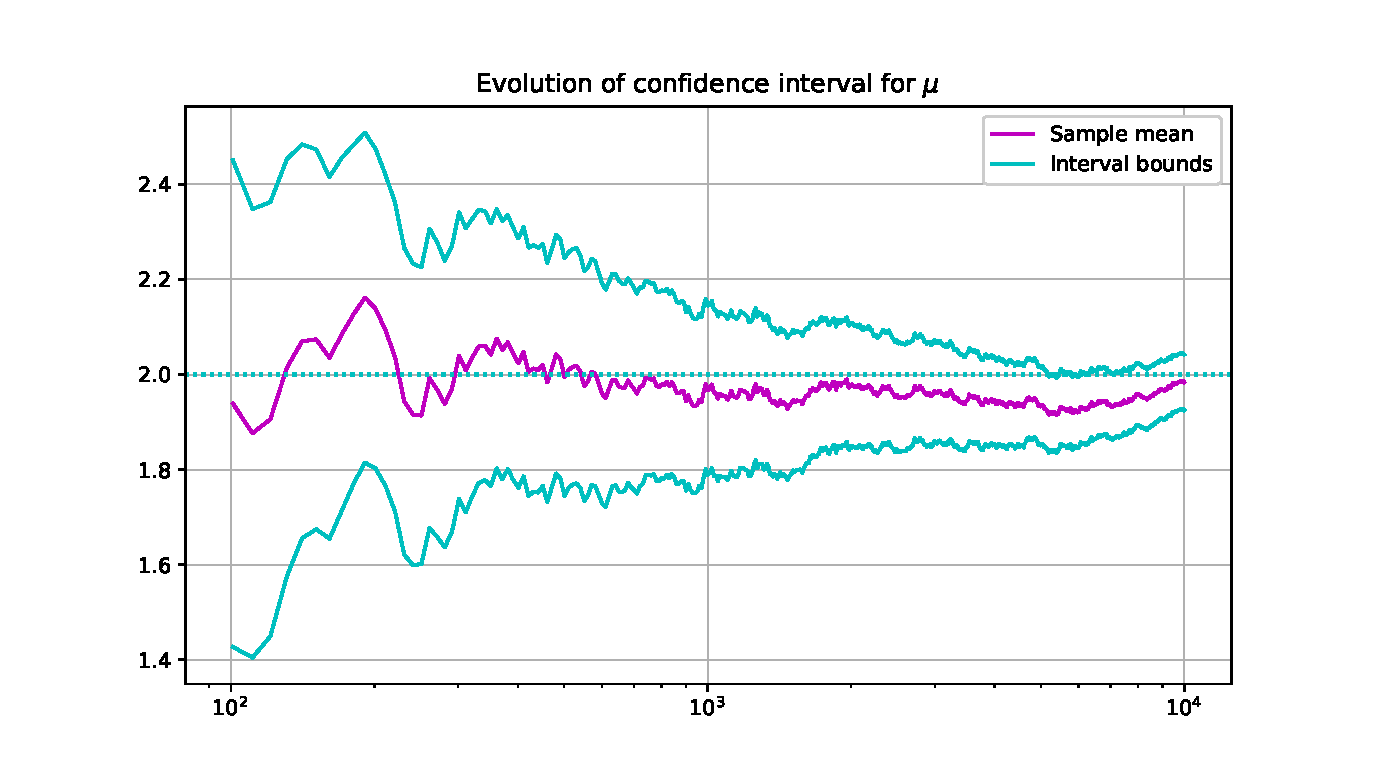
\includegraphics[width=0.9\linewidth]{images/norm-mu-conf.eps}
    \caption{Доверительные интервалы для выборочного среднего выборки из $\mathcal{N}(2,3^2)$ в зависимости от размера выборки.}
    \label{fig:norm-mu-conf}
\end{figure}

\begin{figure}[H]
    \centering
    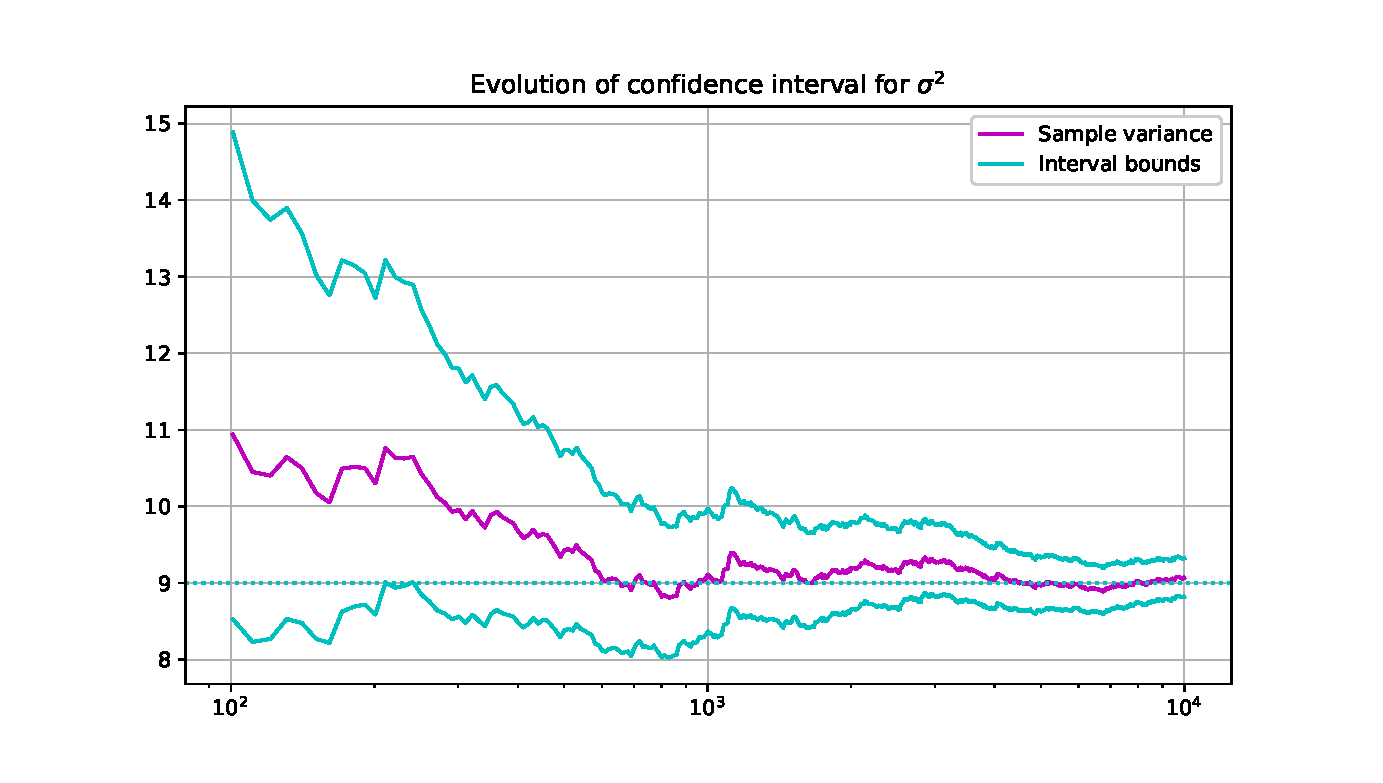
\includegraphics[width=0.9\linewidth]{images/norm-sigma-conf.eps}
    \caption{Доверительные интервалы для выборочной дисперсии выборки из $\mathcal{N}(2,3^2)$ в зависимости от размера выборки.}
    \label{fig:norm-sigma-conf}
\end{figure}

\subsection{Распределение суммы элементов распределения Коши}

\begin{definition}
Характеристической функции случайной величины $X$ называется
$$
\phi(t)=\mathbb Ee^{itX},\quad t\in\mathbb R.
$$
\end{definition}

Рассмотрим $X_1,X_2,\dots\sim C(a,b)$, где $a$ - параметр сдвига, $b>0$ - параметр масштаба. Как известно, плотность распределения Коши задаётся в виде
$$
\dfrac{1}{\pi b\left(1 + (\frac{x-a}{b})^2 \right)}.
$$
Характеристическая функция $\xi\sim C(0,1)$ равна
$$
\varphi_\xi(t) = \int_{-\infty}^{+\infty}e^{itx}\dfrac{dx}{\pi(1+x^2)} = e^{-|t|}.
$$
Используем её для вычисления характеристической функции $X_1$.
$$
\begin{aligned}
\varphi_{X_1}(t) &= \int_{-\infty}^{+\infty}e^{itx}\dfrac{dx}{\pi b\left(1 + (\frac{x-a}{b})^2 \right)} =
\begin{vmatrix}
\begin{array}{c}
x=yb + a \\
dx = bdy
\end{array}
\end{vmatrix} = \\
&= e^{iat}\int_{-\infty}^{+\infty} e^{itby} \dfrac{dy}{\pi(1+y^2)} = e^{iat - b|t|}.
\end{aligned}
$$
Рассмотрим $Y=\frac{S_n}{n} = \frac{\sum_{i=1}^nX_i}{n}$. Тогда
$$
\begin{aligned}
\varphi_Y(t) &= \mathbb{E}e^{itY} = \mathbb{E}\exp\left\{it \frac{\sum_{i=1}^nX_i}{n} \right\} = \left\{ \text{н.о.р.с.в.} \right\} = \\
&= \left( \mathbb{E}\exp\left\{i\frac{t}{n}X_1 \right\} \right)^n = \left( \varphi_{X_1}\left(\frac{t}{n}\right) \right)^n = e^{iat - b|t|}.
\end{aligned}
$$
Таким образом, $Y\sim C(a,b)$. Эмпирически убедимся в этом на рисунке \ref{fig:cauchy-sum}.

\begin{figure}[H]
    \centering
    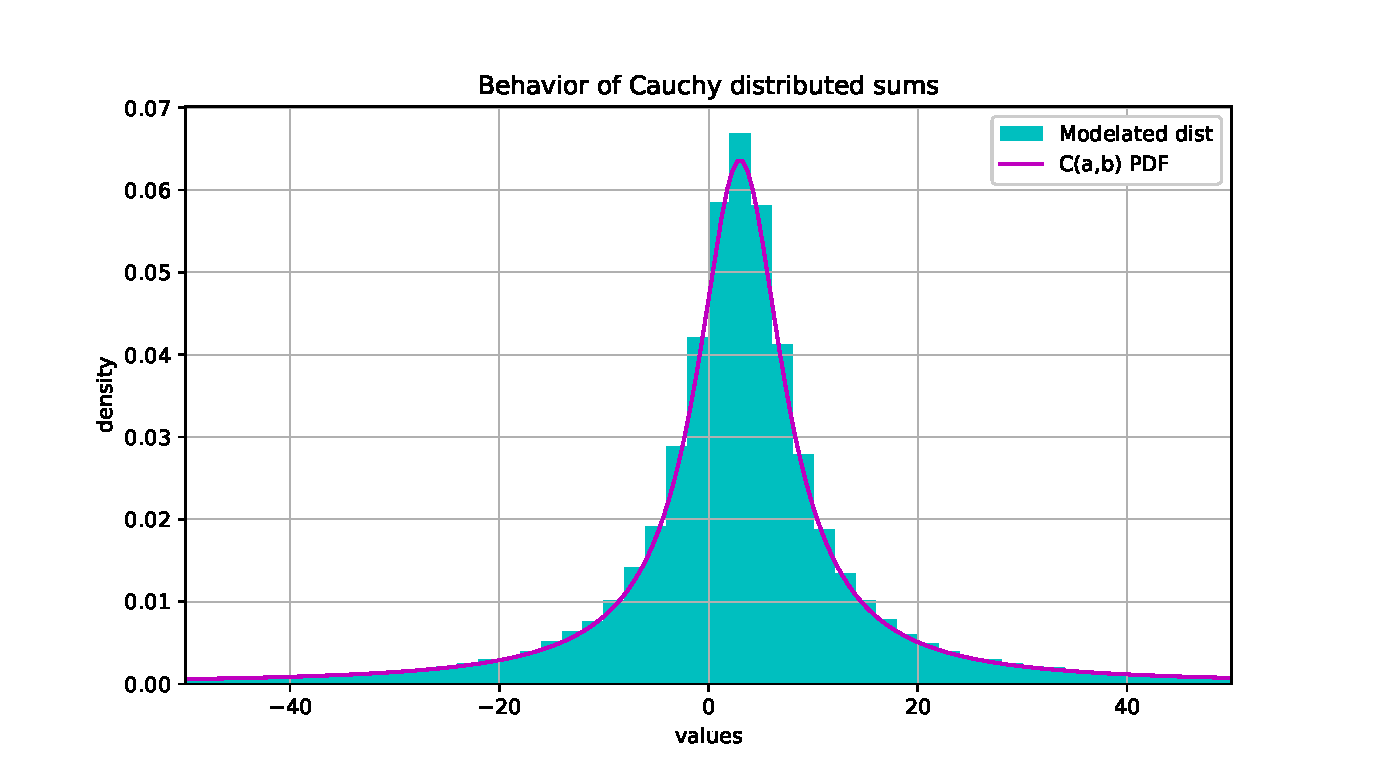
\includegraphics[width=0.9\linewidth]{images/cauchy-sum.eps}
    \caption{Распределение суммы случайных величин $\mathrm{C}(3,5)$.}
    \label{fig:cauchy-sum}
\end{figure}

\section{Задание 6}

\subsection{Условие}

\begin{enumerate}
\item Вычислить следующий интеграл:
$$
I = \int_{-\infty}^{\infty}\int_{-\infty}^{\infty}\cdots\int_{-\infty}^{\infty}
\dfrac{e^{-(x_1^2+x_2^2+\dots+x_{10}^2 + \frac{1}{2^7\cdot x_1^2\cdots x_{10}^2})}}{x_1^2\cdot\dots\cdot x_{10}^2}
dx_1dx_2\dots dx_{10}
$$
\begin{itemize}
\item Методом Монте-Карло,
\item Методом квадратур, сводя задачу к вычислению собственного интеграла Римана.
\end{itemize}
\item Оценить точность вычислений для каждого из двух случаев.
\end{enumerate}

\subsection{Вычисление интеграла}

Можно заметить, что интеграл существует, и он представим в виде
$$
\begin{aligned}
I &= \pi^5\int_{-\infty}^{\infty}\int_{-\infty}^{\infty}\cdots\int_{-\infty}^{\infty}
\underbrace{\dfrac{1}{\sqrt{\pi}^{10}}\exp\left\{ -\sum_{i=1}^{10}x_i^2 \right\}}_{p_{\xi}(x_1,x_2,\dots,x_{10})} \cdot 
\underbrace{\dfrac{\exp\left\{- \frac{1}{2^7\cdot\prod_{i=1}^{10}x_i^2} \right\}}{\prod_{i=1}^{10}x_i^2}}_{f(x_1,x_2,\dots,x_{10})}
dx_1dx_2\dots dx_{10} = \\
&= \pi^5\int_{-\infty}^{\infty}\int_{-\infty}^{\infty}\cdots\int_{-\infty}^{\infty}f(x_1,x_2,\dots,x_{10})p_{\xi}(x_1,x_2,\dots,x_{10})
dx_1dx_2\dots dx_{10},
\end{aligned}
$$
что равняется $\mathbb{E}[f(\xi)]$, где $\xi$ - случайный вектор, компонентами которого являются независимые нормально распределенные случайные величины с параметрами $\mu=0, \sigma^2=\frac{1}{2}$.

Независимость следует из того, что совместная плотность представима в виде произведения плотностей отдельных компонент:
$$
p_{\xi}(x_1,x_2,\dots,x_{10}) = p_{\xi_1}(x_1)p_{\xi_2}(x_2)\cdots p_{\xi_{10}}(x_{10}),
$$
где $\xi=(\xi_1,\xi_2,\dots,\xi_{10}),~ \xi_i\sim\mathrm{N}(0,\frac{1}{2}),~ i=\overline{1,10}$.

Рассмотрим $\eta_i=f(\xi),i=\overline{1,n}$ - н.о.р.с.в. \
Согласно теореме о законе больших чисел
$$
\dfrac{\eta_1 + \eta_2 + \dots + \eta_n}{n} \stackrel{\mathbb{P}}{\longrightarrow} \mathbb{E}\eta_1,~ n\to\infty.
$$

Альтернативно воспользуемся методом прямоугольников. Для этого рассмторим замену $x_i = \operatorname{tg}(\frac{\pi}{2}\varphi_i),~i=\overline{1,10}$. Определитель якобиана равен
$$
|J| = \left( \dfrac{\pi}{2} \right)^{10} \left(\prod^{10}_{i=1}\cos\left(\frac{\pi}{2}\phi_i\right)\right)^{-1}.
$$
Интеграл равен
$$
\begin{aligned}
I &= \left( \dfrac{\pi}{2} \right)^{10}\int_{-1}^1\int_{-1}^{1}\cdots\int_{-1}^1 \theta(\phi_1,\phi_2,\dots,\phi_{10})d\phi_1d\phi_2\dots d\phi_{10}, \\
\theta(\phi_1,\phi_2,\dots,\phi_{10}) &= \dfrac{1}{\prod^{10}_{i=1}\sin^2\left(\frac{\pi}{2}\phi_i\right)}
\exp\left\{ -\left( \sum_{i=1}^{10}\operatorname{tg}^2\left(\frac{\pi}{2}\varphi_i\right) + \dfrac{1}{2^7}\prod^{10}_{i=1}\operatorname{ctg}^2\left(\frac{\pi}{2}\varphi_i\right) \right) \right\}.
\end{aligned}
$$

Подинтегральная функция $\theta(\overline\varphi)$ обладает следующими свойствами.
- $\theta(\overline\varphi)$ четна по каждому аргументу.
- $\theta(\overline\varphi)$ инвариантна относительно перестановки аргументов $\phi_i\mapsto\phi_j,i\neq j$.

Первое свойство позволяет свести пределы интегрирования к $[0,1]$, т.е.
$$
\begin{aligned}
I &= \pi^{10} \int_{0}^1\int_{0}^{1}\cdots\int_{0}^1 \theta(\phi_1,\phi_2,\dots,\phi_{10})d\phi_1d\phi_2\dots d\phi_{10}.
\end{aligned}
$$
Введём равномерную сетку на $(0,1)^{10}$.
$$
T = \{ (t^1_{i_1}, t^2_{i_2}, \dots, t^{10}_{i_{10}})~|~t^k_{i_k} = \dfrac{i_k + \frac{1}{2}}{N+1},~ i_k=\overline{1,N},~ k=\overline{1,10} \}.
$$
Тогда
$$
\begin{aligned}
I &\approx \left( \dfrac{\pi}{N} \right)^{10} \sum_{i=1}^{N}\dots\sum_{i_{10}=1}^{N} \theta(t^1_{i_1}, t^2_{i_2}, \dots, t^{10}_{i_{10}}) = \\
&= \left( \dfrac{\pi}{N} \right)^{10} \sum_{i=1}^{N}\dots\sum_{i_{10}=1}^{N}
\theta\left(\dfrac{i_1 + \frac{1}{2}}{N+1}, \dfrac{i_2 + \frac{1}{2}}{N+1}, \dots, \dfrac{i_{10} + \frac{1}{2}}{N+1} \right).
\end{aligned}
$$
В силу инвариантности под знаками суммирования возникают равные значения для перестановок одного и того же набора индексов. \
Для каждого набора различных индексов таких перестановок всего $10!$. \
Для набора индексов, где встречаются равные значения, таких перестановок всего существует
$$
\frac{10!}{m_1!m_2!\cdots m_{N}!},
$$
где $m_k!$ - число индексов в наборе $(i_1,i_2,\dots,i_{10})$, равных $k$.

Таким образом,
$$
I \approx \left( \dfrac{\pi}{N} \right)^{10} \sum_{1\leqslant i_0\leqslant i_1\leqslant\dots \leqslant i_{10}\leqslant N}
\frac{10!}{m_1!m_2!\cdots m_N!}\cdot
\theta\left(\dfrac{i_1 + \frac{1}{2}}{N+1}, \dfrac{i_2 + \frac{1}{2}}{N+1}, \dots, \dfrac{i_{10} + \frac{1}{2}}{N+1} \right).
$$

\subsection{Оценка точности вычисления}

Оценим точность вычислений эмпирически. Как можно заметить, значение интеграла, вычисленного по методу Монте-Карло находится в окрестности числа 125 (рисунок \ref{fig:integ-monte-carlo}). При этом значение, вычисленное квадратурным методом, зависит как квадратный корень от размера дискретизации (рисунок \ref{fig:integ-rectangular}) и с увеличением таковой стремится к тому же числу.

Найдём аналитическую оценку скорости сходимости для метода Монте-Карло. Из теоремы о ЗБЧ для последовательности независимых одинаково распределенных случайных величин с конечными первым и вторым моментами: $\mathbb X_i = a,\mathbb D X_i = \sigma^2$ следует, что
$$
\overline{X}_n = \frac{1}{n}\sum\limits_{i=1}^nX_i, \quad
\mathbb{E}[\overline{X}_n - a ]^2 = \frac{\sigma}{\sqrt{n}}.
$$
Таким образом, скорость сходимости составляет $\frac{\sigma}{\sqrt{n}}$ (достаточно медленная).
Отметим, что при этом метод Монте-Карло является универсальным.

\begin{figure}[H]
    \centering
    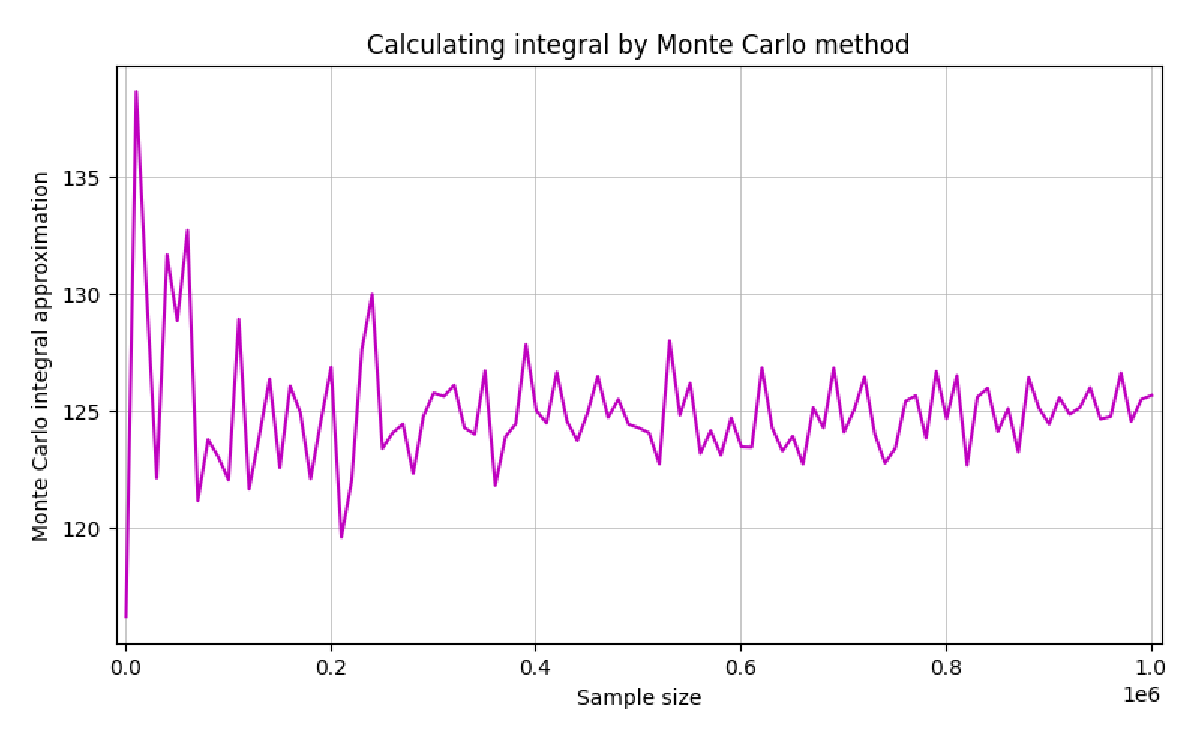
\includegraphics[width=0.9\linewidth]{images/integ-monte-carlo.eps}
    \caption{Приближенное значение интеграла, полученного методом Монте-Карло, в зависимости от размера выборки.}
    \label{fig:integ-monte-carlo}
\end{figure}

\begin{figure}[H]
    \centering
    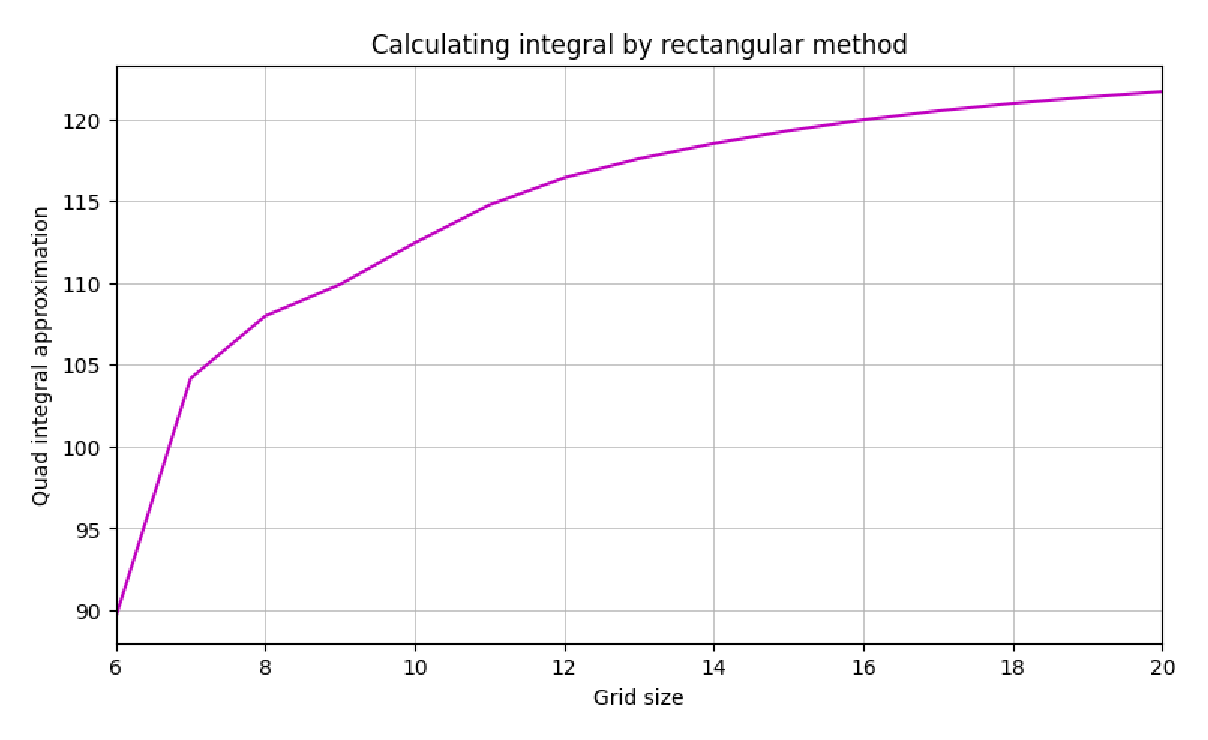
\includegraphics[width=0.9\linewidth]{images/integ-rectangular.eps}
    \caption{Приближенное значение интеграла, полученного методом квадратур, в зависимости от размера дискретной сетки.}
    \label{fig:integ-rectangular}
\end{figure}

\chapter{Вторая часть практикума}

\section{Задание 7}

\subsection{Условие}

\begin{enumerate}
\item Методом случайного поиска найти минимальное значение функции $f$ на множестве $A = \{(x_1,x_2):~x_1^2+x_2^2\leqslant 1\}$, где
$$
f(x_1,x_2) = x_1^3\sin\frac{1}{x_1} + 10x_1x_2^4\cos\frac{1}{x_2},\quad x_1,x_2\neq0.
$$
При $x_1=0$ или $x_2=0$ функция доопределяется по непрерывности.

\item Методом имитации отжига найти минимальное значение функции Розенброка $g$ в пространстве $\mathbb{R}^2$, где
$$
g(x) = (x_1-1)^2 + 100(x_2-x_1^2)^2.
$$

\item Оценить точность и сравнить результаты со стандартными методами оптимизации.
\end{enumerate}

\subsection{Метод случайного поиска}

Метод случайного поиска минимального значения функции $f(x)$ на множестве $A$:
\begin{enumerate}
\item Смоделировать выборку размера $n$ точек $x\sim\mathrm{U}\{A\}$ (равномерно распределены на множестве A).
\item Выбрать ту реализацию случайной величины, на которой достигается наименьшее значение.
\end{enumerate}

Данная функция $f(x)=x_1^3\sin\frac{1}{x_1}+10x_1x_2^4\cos\frac{1}{x_2}$ обладает свойствами
\begin{enumerate}
\item $f(x_1,-x_2)=f(x_1,x_2)$ (чётность по $x_2$).
\item $f(-x_1,0)=f(x_1,0)=x_1^3\sin\frac{1}{x_1}$.
\item $f(0,0)=0$.
\end{enumerate}

Следовательно, если $x^*=(x_1^*,x_2^*)$ доставляет минимум функции, то $(x_1^*,-x_2^*)$ также доставляет минимум. \
Минимум меньше нуля, ведь $f(0.123, 0.123) < 0$ (проверяется численно). \
Следовательно, функция $f$ имеет хотя бы две точки глобального минимума.

По условию задачи множество $A$ - круг единичного радиуса на плоскости $(x_1,x_2)$. Пусть $x=(x_1,x_2)\sim\mathrm{U}(A)$. По определению для любого борелевского множества $M$ выполняется ($\mu$ - мера Лебега на плоскости)
\begin{multline*}
\mathbb{P}\left( (x_1,x_2)\in M \right) = \dfrac{\mu (M)}{\mu (A)} = \dfrac{1}{\pi}\iint\limits_M dt_1dt_2 = \begin{vmatrix}
t_1 = r\cos\alpha \\
t_2 = r\sin\alpha
\end{vmatrix} =\\
= \dfrac{1}{\pi}\iint\limits_M rdrd\alpha = \iint\limits_M d(r^2)d\left(\frac{\alpha}{2\pi}\right).
\end{multline*}

Следовательно, будем моделировать
$$
\begin{cases}
x_1 = \sqrt{\omega}\cos\alpha \\
x_2 = \sqrt{\omega}\sin\alpha
\end{cases}
$$
где $\omega\sim\mathrm{U}[0,1], \alpha\sim\mathrm{U}[0,2\pi]$.



\subsection{Метод имитации отжига}

\subsection{Сравнение методов со стандартными методами оптимизации}

\subsubsection{Метод случайного поиска}

Пусть $\varepsilon>0$ - наперед заданная точность вычислений. Пусть $x^*=(x_1^*,x_2^*)$ доставляет минимум функции $f(x_1,x_2)$. \
Оценим точность работы алгоритма при помощи многомерной теоремы Лагранжа
$$
|f(x) - f(x^*)| \leqslant \max\limits_A 
\sqrt{\left(\dfrac{\partial f}{\partial x_1}\right)^2 + \left(\dfrac{\partial f}{\partial x_2}\right)^2} \cdot || x - x^* ||.
$$

Справедливы следующие оценки
$$
\begin{aligned}
\left|\dfrac{\partial f}{\partial x_1}\right| &= \left| 3x_1^2\sin\frac{1}{x_1} - x_1\cos\frac{1}{x_1} + 10x_2^4\cos\frac{1}{x_2}  \right| \leqslant 14. \\
\left|\dfrac{\partial f}{\partial x_2}\right| &= \left| 40x_1x_2^3\cos\frac{1}{x_2} + 10x_1x_2^2\sin\frac{1}{x_2} \right| \leqslant 50.
\end{aligned}
$$

Далее выберем окрестность радиуса $\delta$: $B_\delta(x^*)=\{ x: ||x-x^*||\leqslant \delta \}$. \
Пусть $p$ - вероятность того, что в $B_\delta(x^*)$ находится хотя бы одна точка выборки.


\section{Задание 8}

\begin{enumerate}

\item Применить метод Монте-Карло к решению первой краевой задачи для двумерного уравнения Лапласа в единичном круге
$$
\begin{cases}
\Delta u = 0,(x,y)\in D \\
u\vert_{\delta D} = f(x,y) \\
u\in C^2(D), f\in C(\delta D) \\
D=\{(x,y)\in\mathbb{R}^2: x^2+y^2\leqslant 1 \}
\end{cases}
$$

\item Для функции $f(x,y) = x^2-y^2$ найти аналитическое решение и сравнить с полученным по методу Монте-Карло.

\end{enumerate}

\subsection{Метод Монте-Карло для уравнения Лапласа}

Будем решать задачу не в единичном круге, а в единичном квадрате. Решение при этом не изменится, ведь $x^2-y^2$ --- единственное решение поставленной задачи в единичном круге, которое является непрерывным. После работы алгоритма выберем только те точки, которые лежат в единичном круге.

Введём сетку на единичном квадрате $|x|\leqslant1, |y|\leqslant1$.

Конечно-разностная схема для уравнения Лапласа представима в виде
$$
u(P) = \dfrac{1}{4}\left( u(P_1) + u(P_2) + u(P_3) + u(P_4) \right).
$$

\subsection{Сравнение численного результата с аналитическим решением}

Функция $f(x,y)=x^2-y^2$ удовлетворяет $\Delta u=0$. Для внешней задачи Дирихле условием регулярности является ограниченность функции $u$. Функция $f=u$ является ограниченной, следовательно, данное уравнение имеет единственное решение, равное $x^2-y^2$.

\section{Задание 9}

\section{Задание 10}

\section{Задание 11}

\begin{thebibliography}{99}

\bibitem{smirnov}
\textit{Смирнов~С.\,Н.}
Лекции по стохастическому анализу.~2023-2024.

\bibitem{shiryaev-1}
\textit{Ширяев~А.\,Н.}
Вероятность, Кн. 1 - \textit{М.:МЦНМО}, 2021.

\bibitem{devroye}
\textit{Devroye~L.}
Non-uniform random variate generation, \textit{Springer-Verlag, New York}, 1986.

\bibitem{kropacheva-tihomirov}
\textit{Кропачева~Н.\,Ю., Тихомиров~А.\,С.}
Моделирование случайных величин: Метод. указания, \textit{Великий Новгород}, 2004.

\bibitem{nekrutin}
\textit{Некрутин~В.\,В.}
Моделирование распределений, 2014.

\bibitem{buslenko}
\textit{Бусленко~Н.\,П., Соболь~И.\,М., Срагович~В.\,Г., Шрейдер~Ю.\,А.}
Метод статистических испытаний, 1961.

\bibitem{feller-1}
\textit{Феллер~В.}
Введение в теорию вероятностей и ее приложения, Том 1, \textit{М.: Мир}, 1964.

\bibitem{feller-2}
\textit{Феллер~В.}
Введение в теорию вероятностей и ее приложения, Том 2, \textit{М.: Мир}, 1967.

\bibitem{kalman}
\textit{Kalman~R.\,E.}
A New Approach to Linear Filtering and Prediction Problems, \textit{Research Institute for Advanced Study, Baltimore, Md.}, 1960.

\bibitem{lewis}
\textit{Lewis P.\,A.\,W., Shedler G.\,S.}
Simulation of Nonhomogeneous Poisson Processses by Thinning, 1979.

\bibitem{ostrem}
\textit{Острем К.\,Ю.}
Введение в стохастическую теорию управления, \textit{М.: Мир}, 1973.

\end{thebibliography}

\end{document}
